\documentclass[conference]{IEEEtran}
\IEEEoverridecommandlockouts
% The preceding line is only needed to identify funding in the first footnote. If that is unneeded, please comment it out.
\usepackage{cite}
\usepackage{amsmath,amssymb,amsfonts}
\usepackage{graphicx}
\usepackage{textcomp}
\usepackage{xcolor}
\usepackage{subfig}
\usepackage{algorithm}
\usepackage{algpseudocode}
\usepackage{diagbox}
\usepackage{footnote}
\usepackage{bbding} %\Checkmark \XSolid
% to be able to draw some self-contained figs
\usepackage{tikz}
% inlined bib file
\usepackage{filecontents}
\usepackage{flushend}

\algrenewcommand\textproc{}% Used to be \textsc
\newcommand{\pushcode}[1][1]{\hskip\dimexpr#1\algorithmicindent\relax}

\def\BibTeX{{\rm B\kern-.05em{\sc i\kern-.025em b}\kern-.08em
    T\kern-.1667em\lower.7ex\hbox{E}\kern-.125emX}}
\begin{document}

\title{Lock Violation for Fault-tolerant Distributed Database System}


\author{\IEEEauthorblockN{Hua Guo}
\IEEEauthorblockA{\textit{School of Information} \\
\textit{Renmin University of China}\\
Beijing, China \\
guohua2016@ruc.edu.cn}
\and
\IEEEauthorblockN{Xuan Zhou}
\IEEEauthorblockA{\textit{School of Data Science And Engineering} \\
\textit{East China Normal University}\\
Shanghai, China \\
xzhou@dase.ecnu.edu.cn}
\and
\IEEEauthorblockN{Le Cai}
\IEEEauthorblockA{
%\textit{} \\
\textit{Alibaba Group}\\
US \\
le.cai@alibaba-inc.com}

}

\maketitle

\begin{abstract}
Modern distributed database systems scale horizontally by sharding its data on a large number of nodes.
To achieve fault tolerance, most of such systems build their transactional layers on a replication layer,
which employs a consensus protocol to ensure data consistency.
Synchronization among replicated state machines thus becomes a major overhead of transaction processing.
Without careful design, synchronization could amplify transactions' lock duration and impair the system's scalability.
Speculative techniques, such as Controlled Lock Violation (CLV) and Early Lock Release (ELR), prove to be effective in shortening lock duration and boosting the performance of transaction processing.
An intuitive idea is to use these techniques to optimize geo-replicated and distributed databases(GDDB).
In this paper, we show that a naive application of speculation is often unhelpful in a distributed environment.
Instead, we introduce Distributed Lock Violation (DLV), a specialized speculative technique for geo-replicated distributed databases.
DLV minimizes the cost of conducting lock violation so that it can achieve good performance without incurring severe side-effects.
\end{abstract}

\begin{IEEEkeywords}
Database System, Distributed Transaction, Locking, High Availability
\end{IEEEkeywords}

\section{Introduction}

Modern distributed database systems scale out by partitioning data across multiple nodes, so that it can run transactions on multiple servers in parallel to increase throughput.
When a transaction needs to access multiple partitions, it has to employ a coordination protocol to ensure atomicity.
It is commonly known that such distributed transactions can lead to significant performance degradation.
This is mainly due to the following reasons\cite{Calvin:conf/sigmod/ThomsonDWRSA12}:

1. Coordinated commit requires a chatty protocol (e.g., Two-Phase Commit), which introduces tremendous network overheads;

2. Message transmission overlaps with the critical path of transaction commit, which worsens the contention among transactions.

These issues can be more serious for geo-replicated databases, which face increased network overheads.
The replication layer of a geo-replicated database often uses a Paxos-like consensus protocol to ensure consistency among replicas.
This introduces an additional amount of message transmission, which further increases the duration of transactions.
To facilitate replication, we usually split data into small chunks and replicate each chunk independently.
As a result, cross-chunk transactions (rather than cross-partition transactions) all become distributed transactions.
This makes distributed transactions even more inevitable.

\begin{figure}[htbp]
  \centerline{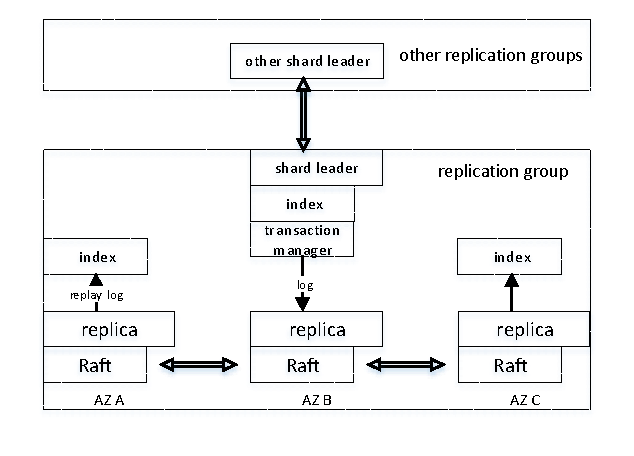
\includegraphics[scale=0.8]{figure/architecture.pdf}}
  \caption{Typical architecture of GDDB}
  \label{fig:architecture}
\end{figure}

Fig.    \ref{fig:architecture} presents the typical architecture of GDDB.
The database partitions its data into many chunks.
For each chunk, the replication layer replicates its data to several Availability Zones (AZ) \cite{Aurora:conf/sigmod/VerbitskiGSCGBM18}.
Among the available zones, the replication layer employs a consensus protocol to shield data consistency.

As discussed in some previous works \cite{Calvin:conf/sigmod/ThomsonDWRSA12}\cite{Tapir:conf/sosp/ZhangSSKP15}\cite{Janus:conf/osdi/MuNLL16},
this architecture has to rely on a two-layer protocol (which integrates the commit protocol and the consensus protocol) to ensure correctness of transactions.
It may fail to scale when confronted with a highly contended workload.


\begin{figure}[htbp]
  \centerline{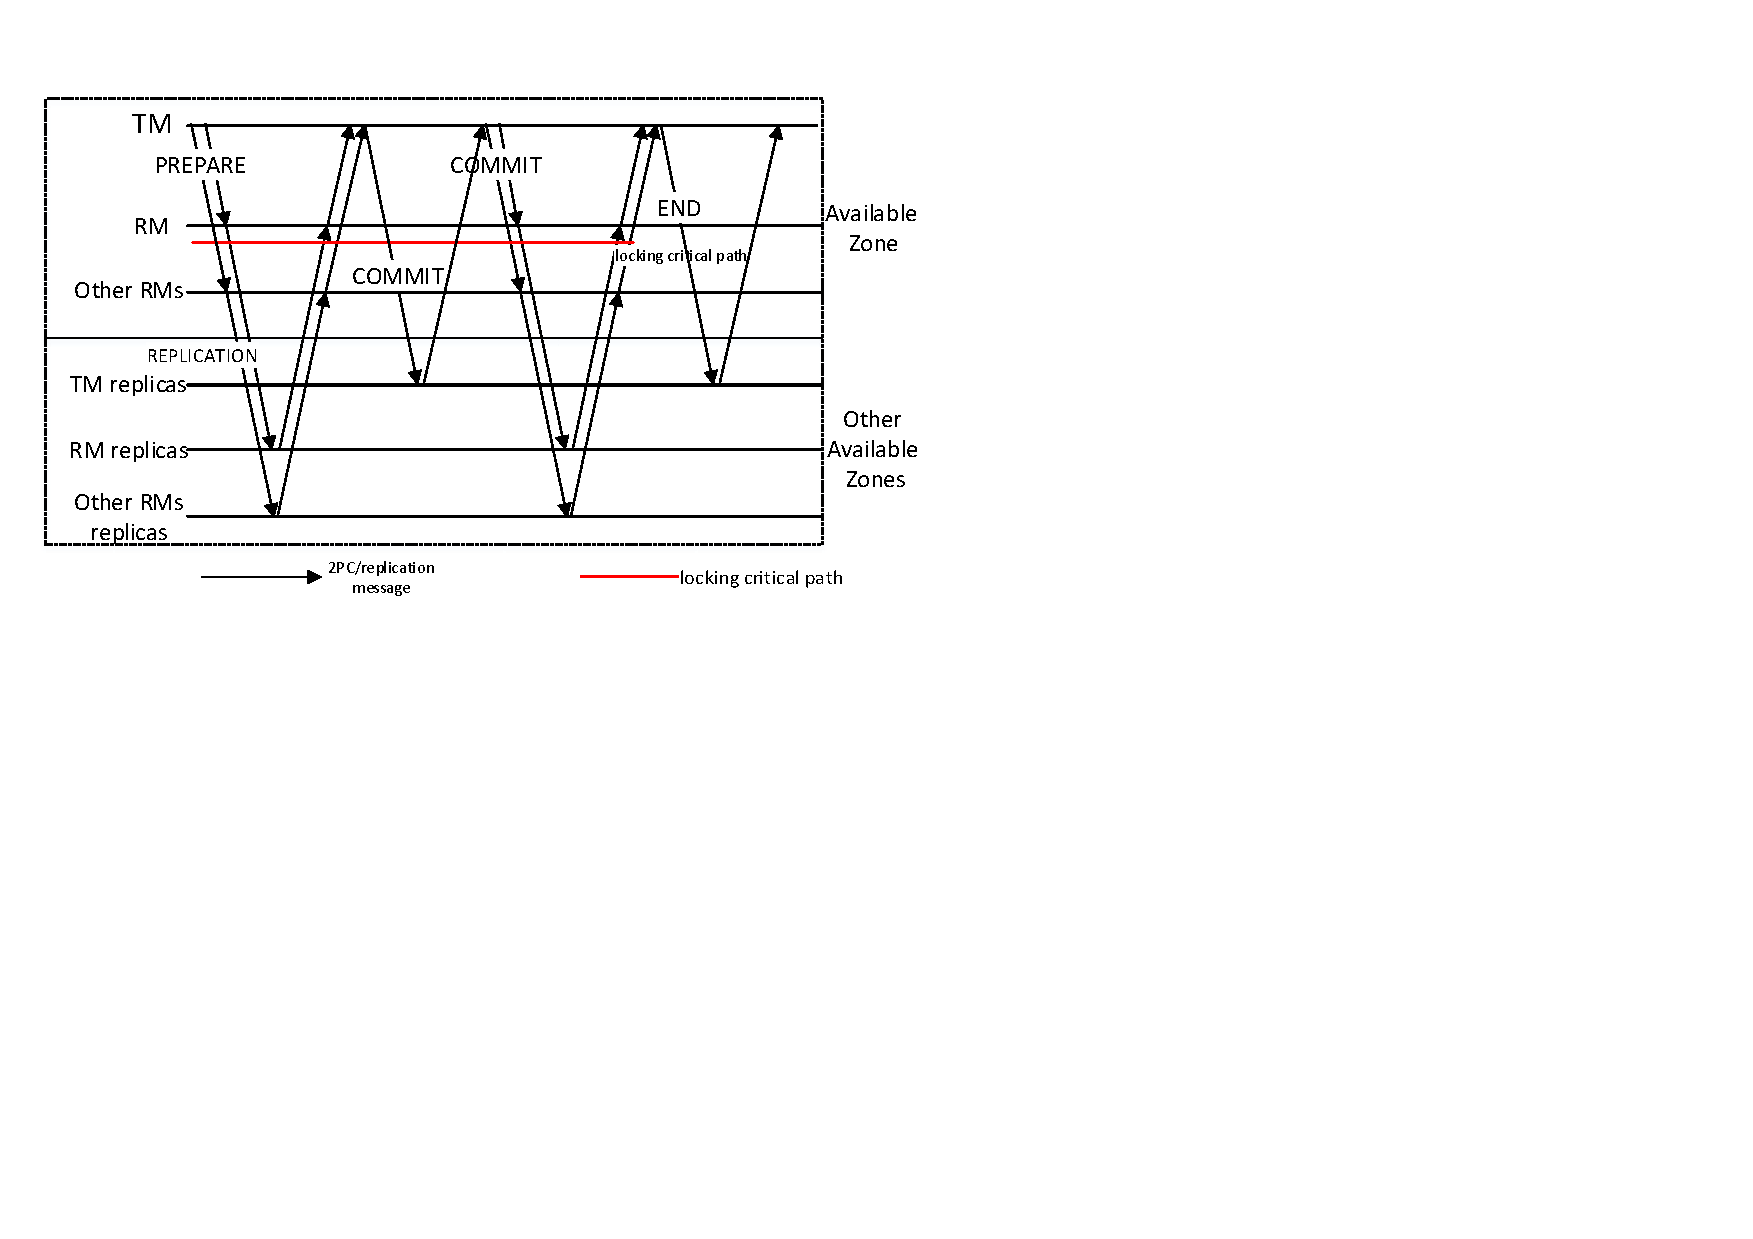
\includegraphics[scale=0.60]{figure/message_flow.pdf}}
  \caption{The message flow and lock holding critical path when the DBMS uses S2PL for concurrency control and 2PC as the commit protocol.
The dash arrow lines represent the messages introduced by Distributed Lock Violation (DLV). The red lines represent the critical paths of S2PL.
The green dash lines represent the critical paths of DLV.}
  \label{fig:message_flow}
\end{figure}

Looking more closely,the main obstacle is that the combination of is that the commit and consensus protocols may enlarge the timespan of the critical paths in transaction processing.
This significantly amplifies the chance of contention.
This architecture supports a wide range of transaction processing methods.
Most industrial data systems choose this two-layer architecture, including Google Spanner \cite{Spanner:conf/osdi/CorbettDEFFFGGHHHKKLLMMNQRRSSTWW12}\cite{Spanner:conf/sigmod/BaconBBCDFFGJKL17},
NuoDB \cite{NuoDB}, CockroachDB \cite{CockroachDB}, TiDB \cite{TiDB}, etc.

Fig.    \ref{fig:message_flow} shows the message flow of a distributed transaction in such an architecture. We assume that
it uses S2PL for concurrency control and 2PC as the commit protocol, and the replication layer is deployed over a WAN.
When a transaction requests to commit, the \emph{TM (transaction manager)} issues a `prepare' message to each \emph{RM (resource manager)}.
Then, each \emph{RM} replicates its vote (`prepare commit' or `prepare abort') to the corresponding replicas through a consensus protocol, before it
sends its vote to \emph{TM}.
After the \emph{TM} collects all the votes of the \emph{RMs}, it replicated its commit log.
\footnote{Depending on variants of implementations, the TM can choose to persist its decision on its log or not.}
TM broadcasts the decision (`commit' or `abort') to all the \emph{RMs}
.
Once a \emph{RM} receives the final decision from the \emph{TM}, it replicates the decision to the corresponding replicas.
After the consensus of commit or abort reaches, the \emph{RM}
can release the locks it had retained over the accessed data.
Finally, \emph{TM} replicate an end log to finish the transaction and clean the transaction context.


We depict the lock duration by red lines in Fig.    \ref{fig:message_flow}.
As we can see, the lock duration spans multiple messages round trips, including those over the WAN.
Fig.    \ref{fig:log_write_latency} shows the WAN RTT, LAN RTT and disk seek approximate time.
This may severely impair degree of parallelism especially in face of intensive contention.

Speculative techniques, such as Early Lock Release (ELR) \cite{EfficientLocking:conf/vldb/KimuraGK12} and Controlled Lock Violation (CLV)
\cite{CLV:conf/sigmod/GraefeLKTV13}, prove to be effective in optimizing centralized transaction processing.
They can be extended to a distributed environment.

\begin{figure}[htbp]
  \centerline{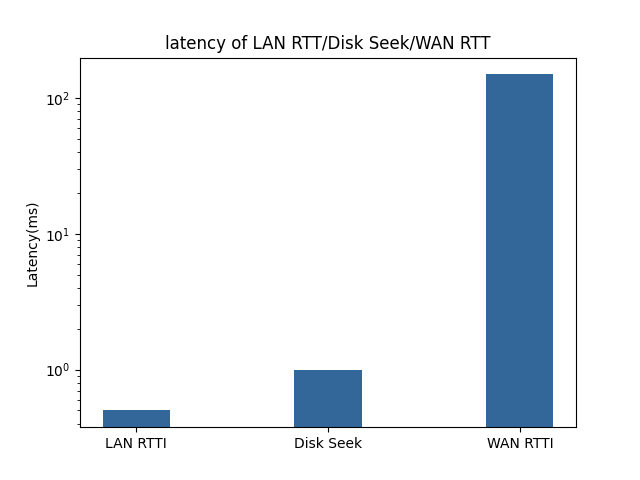
\includegraphics[scale=0.4]{figure/log_write_latency.png}}
  \caption{approximate latency comparison\cite{Latency}}
  \label{fig:log_write_latency}
\end{figure}

Speculative techniques improve concurrency by excluding logging from lock duration.
Transactions on GDDB require much more time to ship and persist logs.

This provides more opportunities for exploiting speculation.
However, the application of speculation in a distributed environment is complex.
Several design choices need to be considered.
For instance, when working with 2PC, we need to decide to violate (or release) lock at which phase.
As some previous work suggested \cite{CLV:conf/sigmod/GraefeLKTV13}, lock violation at the first phase may enable a higher degree of concurrency.
However, dependency tracing and cascade abort may incur excessive overheads.
On the contrary, lock violation at the second phase costs less on in-dependency tracing and cascade abort, while it has to sacrifice a certain amount of concurrency.
%Transaction models, interactive or one-shot transactions, may have different message flow, how different transaction types could benefit from these techniques?
Moreover, not all transactions can benefit from CLV or ELR, e.g., workload with little conflict.
It is unnecessary and even harmful to apply speculation to all cases.


To the best of our knowledge, this is the first experimential study on lock violation of GDDB.
We found that CLV does always not necessarily help of the performance on GDDB.
The reason is that violation serializabile and cascade abort would more likely occur.
In this paper, we propose a technique called Distributed Lock Violation (DLV) to enhance the performance of GDDB.
DLV can harness the most benifit of CLV in GDDB and it minimize the cascade abort penalty and dependency tracing cost.

The remainder of this paper is organized as follows.
Section \ref{sec:relate_work} reviews related work.
In Section III, we explain why a strict schedule is not necessary and may hurt the performance of distributed DBMS.
Section \ref{sec:implement} introduces DLV.
Section \ref{sec:experiments} evaluates DLV and compares it against previous work.
Section \ref{sec:conclusion} concludes this paper.


\section{Relate Work}
\label{sec:relate_work}
%This section introduces the related work of this paper.

\subsection{Transaction Processing on Replicated Databases}
%Recently, there are many scalable DBMS arisen in both academia and industry.
%Most of the systems in this category supports distributed query processing and
%replicate data across several data centers geo-located in different areas for fault tolerance.

Most replicated databases rely on state-machine replication(SMR) to realize high availability.
SMR often uses a consensus protocol to synchronize different replicas.
The synchronization introduces a significant amount of network traffic and becomes a major overhead of replicated database systems.
Paxos \cite{Paxos:journals/tocs/Lamport98}\cite{PaxosSimple:conf/opodis/Lamport02} is the most well known consensus protocol.
To reach a consensus on a single data update in Paxos, it costs two message round trips, one for choosing a proposal and another for proposing the entry.
Multidecree Paxos\cite{Multidecree:journals/csur/RenesseA15} elects a leader as the only proposer to eliminate the first message round trip.
Raft\cite{Raft:conf/usenix/OngaroO14} is a similar consensus protocol to Paxos. As it is more understandable, it is widely used in modern database systems.
In Raft, it costs at least one message round trip to reach a consensus.
Google Spanner \cite{Spanner:conf/osdi/CorbettDEFFFGGHHHKKLLMMNQRRSSTWW12}\cite{Spanner:conf/sigmod/BaconBBCDFFGJKL17},
NuoDB \cite{NuoDB}, CockroachDB \cite{CockroachDB} and TiDB \cite{TiDB} are all geo-replicated DBMSes built upon Paxos or Raft.
They all face heavy costs incurred by data synchronization.

To minimize the cost of synchronization, many techniques have also been proposed.
VoltDB \cite{VoltDB} and Calvin \cite{Calvin:conf/sigmod/ThomsonDWRSA12} employ a deterministic transaction model
to reduce the coordination cost of distributed transactions.
Deterministic scheduling enables active replication, which allows transactions to kickoff synchronization at the earliest possible time.
Tapir \cite{Tapir:conf/sosp/ZhangSSKP15} relaxes the consistency requirements of the replication layer so that it can reduce the message round trips to reach consensus.
Janus \cite{Janus:conf/osdi/MuNLL16} aims to minimize wide-area message round trips
by consolidating the concurrency control mechanism and the consensus protocol.
It uses deterministic serializable graph tracing to ensure the atomicity of transactions.
In a nutshell, Tapir and Janus both co-designed the transaction and replication layers of distributed databases, so that they only need to incur one wide-area message round trip to commit a transaction.
VoltDB, Calvin, Tapir and Janus all impose strict constraints on the implementation of the transaction layer, making them incompatible with existing systems, such as Spanner and CockroachDB.
In contrast, this work focuses on the optimization opportunities in the general implementation of geo-replicated and distirbuted databases (GDDB, as depicted in Fig.    \ref{fig:architecture}).

\subsection{Optimization on Locking based Concurrency Control}
%DBMS use concurrency control(CC) to calculate a serializable schedule for concurrent transactions.
Two-phase locking (2PL) is the most widely used concurrency control mechanism.
As a pessimistic method, 2PL assumes a high likelihood of transaction conflict.
It uses locks to enforce the order of conflicting transactions.
Strict 2PL (S2PL) is a brute force implementation of 2PL. 
It requires a transaction to preserve all its lock until it ends.
As S2PL can easily guarantee transactions' recoverability, many databases choose to use it.
When extending S2PL to distributed databases, the lock holding time will be substantially enlarged, 
as the commit critical path will involve several message round trips.

All S2PL implementations adopt a certain approach to resolve deadlocks.
In the \emph{no-wait}
\cite{EvaluationOfCC:journals/pvldb/HardingAPS17}
approach, a transaction immediately aborts if it fails to place a lock.
Previous works showed that this is a scalable approach in a distributed environment \cite{EvaluationCC1000Cores:journals/pvldb/YuBPDS14}\cite{EvaluationOfCC:journals/pvldb/HardingAPS17},
as it eliminates blocking completely.
However, it works poorly when dealing with high contention workload.
Another approach is \emph{wait-die} \cite{LockNoWait:journals/csur/BernsteinG81}. 
It avoids some false-positive aborts encountered by \emph{no-wait} by utilizing timestamps.
In DLV, we adopt a variant of the wait-die approach.
The \emph{Deadlock detection} approach \cite{LockCC:conf/ds/GrayLPT76} detects deadlock by explicitly tracing wait-for relationship among transactions
While deadlock detection proves effective in centralized database systems\cite{MySQL}\cite{PostgreSQL}.
%it is costly in a distributed environment.
%However, deadlock detection in a distributed environment is highly costly, making it the least favorable approach in our case.

%\subsection{Exploit Speculation and Lock Violation}
To optimize the performance of locking based concurrency control, speculation can be used.
%Similar approaches have been introduced by many previous works.
Early lock release (ELR)
\cite{ELR:dewitt_implementation_1984}\cite{PS2PL:conf/icdt/Soisalon-SoininenY95}
\cite{Aether:journals/pvldb/JohnsonPSAA10}
\cite{EfficientLocking:conf/vldb/KimuraGK12}
\cite{Actor-Oriented-DB:conf/icde/Bernstein18}
is a typical speculative technique.
ELR allows a transaction to release its locks before its commit log is flushed to disk.
It was first proposed by DeWitt et al.\cite{ELR:dewitt_implementation_1984}.
Soisalon-Soininen et al.\cite{PS2PL:conf/icdt/Soisalon-SoininenY95} analyzed its correctness in various settings.
Many other works applied and evaluated ELR in different types of systems \cite{Aether:journals/pvldb/JohnsonPSAA10}\cite{EfficientLocking:conf/vldb/KimuraGK12}\cite{EfficientLocking:conf/vldb/KimuraGK12}\cite{Aether:journals/pvldb/JohnsonPSAA10}.
However, previous works on ELR were largely limited to centralized database systems.

Control lock violation (CLV) \cite{CLV:conf/sigmod/GraefeLKTV13} is a more general speculative technique than ELR and it mainly focuses centralized DB.
It allows certain transactions to ignore certain locks, instead of releasing a lock completely.
CLV has been tested on distributed databases. The results show that it can optimize both phases of two-phase commit.
CLV needs to trace dependency among transactions.
In \cite{CLV:conf/sigmod/GraefeLKTV13}, the authors use a Register and Report (RARA) approach \cite{HeckatonMVCC:journals/pvldb/LarsonBDFPZ11} to implement the tracer.
RARA works well on a centralized database. In a distributed environment, dependency tracing becomes much more costly.
Cascade abort is another side effect of speculation. It can also leads to severe performance downgrade for distributed databases.
%{TODO} In the section of evaluation, we will compare CLV in [11] against our DLV approach.

\section{Scheduling with Lock Violation}
\label{sec:non_strict}

In the following, we describe the basic idea of applying lock violation to transaction scheduling.

\subsection{Preliminaries and Assumptions}
Our scenario is a GDDB, which shards its data by primary keys.
Each data chunk is replicated across several remotely located AZs.
Physiological logs , which record row-level write operations, are transmitted among the AZs to keep the data synchronized.
A consensus protocol is used to prevent the synchronization from going wrong.
We assume that there is a replica leader for each data chunk, which is responsible for coordinating the synchronization process.

We assume that two types of distributed transactions can be conducted on the system. They are known as one-shot and interactive transactions.
Fig.    \ref{fig:transaction_type} shows the message flow during the commit phase of the two types of transactions.
We can see that an interactive transaction costs more message round trips than a one-shot transaction,
as the $TM$ has to explicitly notify the $RM$s that they can prepare to commit.

\begin{figure}[htbp]
    \centering
    \captionsetup[subfigure]{oneside,margin={0.3cm,0cm}}
    \subfloat[one-shot transaction, which does not need to explicitly ask the $RM$s to prepare]
        { 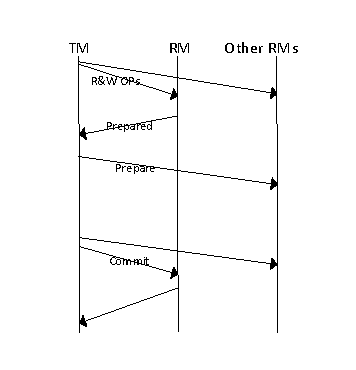
\includegraphics[scale=1] {figure/transaction_oneshot}  \label{fig:transaction_oneshot}  }
    \captionsetup[subfigure]{oneside,margin={0.3cm,0cm}}
    \subfloat[interactive transaction, which has to notify each $RM$ to prepare ]
        { 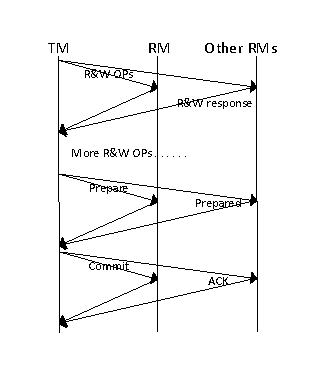
\includegraphics[scale=1]{figure/transaction_interactive} \label{fig:transaction_interactive}}

  \caption{Commit message flows for one-shot and interactive distributed transactions}
  \label{fig:transaction_type}
\end{figure}



\subsection{Concepts of Scheduling}
Before presenting the idea of lock violation, we first review the conceptual model of transaction processing. Most of the contents can be found in previous work, such as \cite{LockNoWait:journals/csur/BernsteinG81}.

\subsubsection{Transaction and History}
Suppose that a distributed database resides on ${n}$ nodes, represented by ${R = \{r_1, r_2, ... r_n\}}$.
A transaction ${T_i}$ can run on any ${m}$ of the ${n}$ nodes ($1 \le m \le n$), represented by  ${S = \{s_1, s_2, ... s_m\} \subseteq R}$,
The transaction ${T_i}$ is composed of a series of operations, 
where each can be a read or a write or other command operation including abort, commit, etc.
Let ${r_i[x]}$ denote that ${T_i}$ reads the record ${x}$. Let ${w_i[x]}$ denote that ${T_i}$ writes on the record ${x}$.
Let ${c_i}$, ${a_i}$, ${p^c_i}$, ${p^a_i}$ denote the commit, abort, prepare-to-commit and prepare-to-abort operations of ${T_i}$ respectively.


A transaction history is a collection ${H = \{h_1, h_2, ..., h_n\}}$, in which
each ${h_u}$ is the local history of $H$ on the node ${s_u}$, which is a sequence of operations issued by different transactions.
For instance, Fig. \ref{fig:strict_example} illustrates a transaction history over three nodes.

\subsubsection{Deterministic and Non-deterministic Abort}
Several reasons can cause a transaction to abort. In general, they can be categorized as:

1. User requested abort. 
These are aborts specified by the program logic (e.g. transaction requires to abort if it has accessed a non-existent record presumed existence).

2. Due to maintaining isolation (e.g., serializability). 
These are aborts commanded by the database system.
Various concurrency control algorithms has different strategies to choose abort transactions.
For a locking scheme using deadlock detection,
the scheduler would choose a transaciton as victim transaction to break circle in wait for graph.

3. Database node failure. 
For simplicity, we assume there are fail-stop failures only.

We call the first two types of abort \emph{deterministic abort} and the last one \emph{non-deterministic abort}.
In a database system, deterministic aborts occur much more frequently than non-deterministic abort.
Therefore, the prices we are willing to pay for the two kinds of abort are very different. 

\subsubsection{Dependencies among Transaction}

There are three kinds of data dependency among transactions, known as \emph{wr-dependency}, \emph{ww-dependency} and \emph{rw-dependency}.
In a local history ${h}$, if ${T_j}$ reads ${T_i}$'s write on ${x}$,
we call it a \emph{write-after-read(wr) dependency} and denote it by ${w_i[x] \rightarrow r_j[x]}$.
Analogically, if ${T_j}$ overwrites ${T_i}$'s write on ${x}$, it is called a \emph{write-after-write(ww) dependency} and denoted by ${w_i[x] \rightarrow w_j[x]}$.
If ${T_i}$ reads ${x}$ before ${T_j}$ writes on ${x}$, it is called a \emph{read-after-write(rw) dependency} and denoted by ${r_i[x] \rightarrow w_j[x]}$.
Based on data dependencies, we can define \emph{commit dependency}. ${T_j}$ has a \emph{commit dependency} on ${T_i}$, written as ${T_i \rightarrow T_j}$, if ${T_j}$ cannot commit prior to ${T_i}$.
In other words, ${T_i}$ aborts, ${T_j}$ has to abort too. ${T_j}$ has a \emph{commit dependency} on ${T_i}$, if and only if ${T_j}$ has a \emph{rw-dependency} on ${T_i}$.
More detail concepts of dependency can be found in \cite{Dependency:conf/sigmod/ChrysanthisR90} \cite{Dependency:conf/sigmod/BilirisDGJR94}
%cite{TODO}

\subsubsection{Relaxation on Corrrect Criteria}

Traditional database systems adopt Strict Two-Phase Locking (S2PL) \cite{DBLP:conf/vldb/Raz92} to ensure the and serializable recoverability of transactions.
Strictness implies that a transaction cannot read a previous write by another transaction that has not committed yet.
Strictness is not a necessary condition for a correct schedule.
Although it simplifies the implementation of a database system, it sacrifices the concurrency of transaction processing.

For instance, the schedule ${H_1}$ of Fig. \ref{fig:strict_example} is serializable and strict. 
(The data dependencies include ${r_1[x] \rightarrow w_3[x]}$, ${w_1[x] \rightarrow r_2[y]}$, ${r_2[y] \rightarrow w_3[x]}$, which are not cyclical.)
In contrast, ${H_2}$ in Fig. \ref{fig:non_strict_example} is serializable but not strict.
In Fig.    \ref{fig:non_strict_example}, there are three records ${x}$, ${y}$, ${z}$, residing on ${s_1}$, ${s_2}$, ${s_3}$ respectively.
${T_1}$ writes ${y}$ and ${x}$.
${T_2}$ reads ${T_1}$'s write on ${x}$ before ${T_1}$ commits.
Transaction ${T_3}$ overwrites ${T_2}$'s write before ${T_2}$ commits.
As we can see, by violating strictness, ${H_2}$  enables a higher degree of concurrency.


\begin{figure}[htbp]
  \centerline{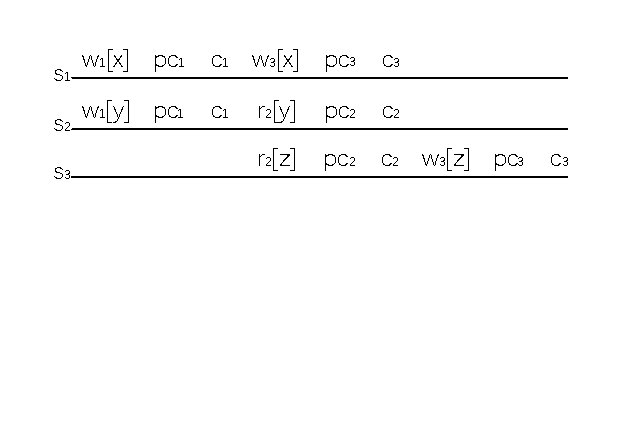
\includegraphics[scale=1]{figure/schedule_strict.pdf}}
  \caption{A strict and serializabile schedule ${H_1}$}
  \label{fig:strict_example}
\end{figure}

\begin{figure}[htbp]
  \centerline{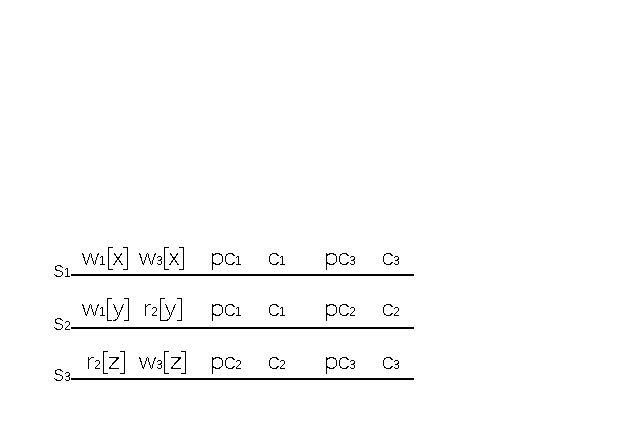
\includegraphics[scale=1]{figure/schedule_non_strict.pdf}}
  \caption{A non-strict but serializabile schedule ${H_2}$}
  \label{fig:non_strict_example}
\end{figure}

\begin{figure}[htbp]
  \centerline{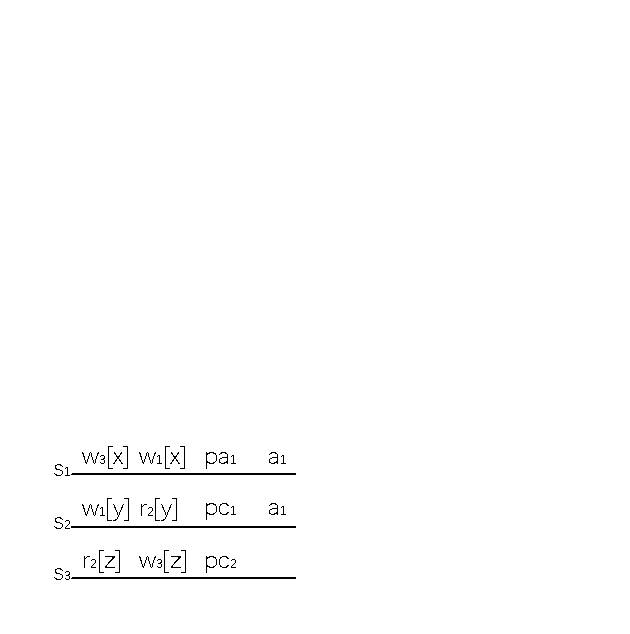
\includegraphics[scale=1]{figure/schedule_not_serializabile.pdf}}
  \caption{Schedule ${H_3}$, ${T_1}$ abort due to non-serializabile}
  \label{fig:schedule_abort_example}
\end{figure}

\begin{figure}[htbp]
  \centerline{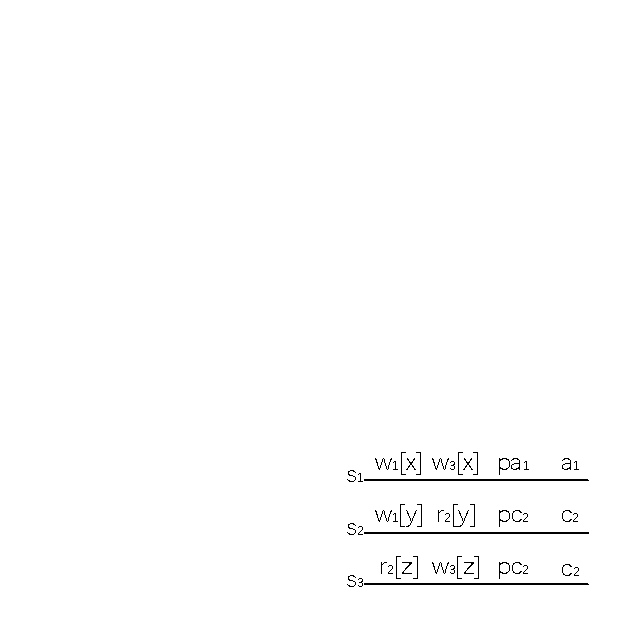
\includegraphics[scale=1]{figure/schedule_not_recoverable.pdf}}
  \caption{Schedule ${H_4}$, ${T_2}$ commit ahead ${T_1}$, non-recoverable anomaly}
  \label{fig:schedule_not_recoverable}
\end{figure}


The drawback of strictness is amplified in a GDDB.
The commit of a transaction in such a database usually involves a lot of work, including multiple rounds of communication across the WAN.
As strictness requires a transaction to hold locks until it finishes committing, this means a substantially lengthened lock holding time. 
This will hurt the performance of distributed transactions severely.
Our basic idea is to develop a serializable but non-strict scheduler to shorten the lock holding time.

Relaxation on strictness will, however, complicate the recovery mechanism.
In a traditional recovery mechanism, such as ARIES, the dependencies among transactions completely comply with the persisting order of their logs. 
This guarantees the recoverability of scheduling, which requires that a transaction cannot commit before the transactions it has commit dependencies on.
When strictness no longer holds, we need other tactics to enforce the commit order, which may incur additional overheads.

\subsection{Lock Violation and Dependency Tracing}

Lock violation is a general technique to enable a non-strict scheduler.
Its basic idea is to allow a transaction to speculatively access data locked by other transactions.
If such speculative data accesses cause a problem, the system should be able to rectify it.

For lock violation to be correct, it should first preserve serializability.
Considering the non-strict schedule ${H_3}$ in Fig. \ref{fig:schedule_abort_example},
it contains three data dependencies:

\begin{center}
${w_3[x] \rightarrow _s w_1[x]}$,
${w_1[y] \rightarrow _s r_2[y]}$
${r_2[z] \rightarrow _s w_3[z]}$
\end{center}

This leads to a circle ${T_1 \rightarrow T_2 \rightarrow T_3 \rightarrow T_1}$, which makes the schedule non-serializable.
${H_3}$ is not possible if we apply S2PL. It becomes possible when lock violation is permitted -- we allow
${T_2}$ to read from uncommitted ${T_1}$, and ${T_1}$ to overwrite uncommitted ${T_3}$.
Therefore, to preserve serializability, we need to prevent the data dependencies from forming a dependency cycle.
Many techniques can be adopted to achieve this, including the \emph{wait-die} strategy mentioned in the related work.

Secondly, a schedule generated by lock violation must be recoverable.
In the schedule ${H_4}$ in Fig.   \ref{fig:schedule_not_recoverable}, due to lock violation,
${T_2}$ reads  ${T_1}$'s write and commits before ${T_1}$.
In this case, if ${T_1}$ later on decides to abort, it is no longer possible to reverse ${T_2}$.
Therefore, ${H_4}$ is not a recoverable schedule.
To ensure recoverability, we need to trace the commit dependencies (i.e., $wr$-dependencies) among +transactions, and force the commit order to comply with the commit dependencies.

Dependencies would be tracing after a lock violation action to maintain serializabile and recoverability.
If we know that ${T_2}$ depends on ${T_1}$, we can hold ${T_2}$'s commit request until ${T_1}$ finishes.
If ${T_1}$ decides to abort, we abort ${T_2}$ too. This is known as \emph{cascade abort}.
Cascade abort can be cause by a deterministic abort or a non-deterministic abort. 

\section{Design of DLV}
\label{sec:implement}

In this section, we present Distributed Lock Violation (DLV).

\subsection {Timing of Lock Violation}


In a distributed transaction, $TM$ assigns work to $RM$. Once the work is done, $TM$ applies 2PC to end the transaction.
In 2PC, both $TM$ and $RM$ need to synchronize with their replicas, to make sure that node failures will not corrupt the data.
Synchronization usually takes a long time, especially when the replicas are located remotely.
DLV aims to prevent data synchronization from coinciding with the lock holding time.

In a GDDB, lock violation can potentially be allowed on two occasions in a transaction.
The first occasion is when the work of the transaction has been completed successfully and the transaction is ready to commit.
We call lock violation at this occasion \emph{late lock violation}. It is only intended to reduce the contention in the commit phases of transactions.
The second occasion is before the transaction is ready to commit. We call lock violation at this occasion \emph{early lock violation}. 
Early lock violation can also fall into two categories: 
violation immediately before an ${RM}$ decides its prepare decision, 
and violation when a transaction is even on-going in this ${RM}$. 


While early lock violation allows us to harness more concurrency, it may cause additional issues. 
First, early lock violation can result in non-serializable schedules. This has been illustrated by ${H_3}$ in Fig.   \ref{fig:schedule_abort_example}.
In contrast, \emph{late lock violation} is safe. If a transaction can only violate the locks of transactions that are ready to commit, it cannot result in cyclic data dependencies.
Second, early lock violation faces a much higher chance of cascade abort. In late lock violation, only non-deterministic aborts can cause cascade abort, as no lock can be violated before deterministic aborts (since the transaction has already been permitted to commit). In early lock violation, all types of aborts can cause cascade abort.


Whether late or early lock violation is adopted, we need to trace the commit dependencies among transactions and make sure they commit in the right order.
In a GDDB, the scheduler should follow the following rules to enforce the commit order.
Given that there is a commit dependency from ${T_j}$ to ${T_i}$,

\begin{enumerate}
  \item ${T_j}$'s $RM$ can persist its `prepare' state (including replication of the state) only if ${T_i}$ has committed;
  \label{rule:prepare}

  \item ${T_j}$'s $TM$ can send out `commit' request only if ${T_i}$ has committed;
  \label{rule:commit}

  \item If ${T_i}$ aborts, ${T_j}$ must also abort too.
  \label{rule:abort}
\end{enumerate}


In \emph{late lock violation}, a transaction allows its lock to be violated only after all $RM$s confirm that they can commit.
Therefore, it requires an additional message round trip between the $TM$ and the $RM$s before the commit starts.
In \emph{early lock violation}, each $RM$ can autonomously decide to when to permit lock violation.
It saves a message round trip but faces a higher chance of cascade abort.
There are four types of late and early lock violation, defined as follows:

\emph{DLV0}: Once a transaction finishes a read or write operation, it allows the lock to be violated immediately;

\emph{DLV1}: After an ${RM}$ finishes its work and before it persists its `prepare' state, it allows its locks to be violated;

\emph{DLV1x}: Once a transaction guarantees that all the ${RM}$s can commit (but before they persist their `prepare' states), it allows all the locks to be violated;

\emph{DLV2}: When a transaction enters the second phase of 2PC, it allows all its locks to be violated.

DLV0 and DLV1 are early lock violation, and DLV1x and DLV2 are late lock violation.
DLV0 allows earlier lock violation than DLV1, while it faces a higher abort rate.
DLV1x releases the locks at the earliest possible time after determining that the transaction can commit. 
However, DLV1x needs an additional message round trip to confirm that all $RM$s are ready to commit.
DLV2 permits lock violation even later than DLV1x.

Fig.~\ref{fig:message_flow} illustrates the commit process of DLV1x.
Before an ${RM}$ persists its `prepare' log, it sends a \emph{Ready} message to notify the ${TM}$ that it is ready to commit or abort.
When the \emph{TM} collects all \emph{RM}s' \emph{Ready} messages, it sends \emph{Violate} messages to notify all the $RM$s that their locks can be violated.
An interactive transaction can combine these messages with the messages of the last operations on $RM$s.
For a one-shot transaction, this additional message round trip cannot be avoided.
Nevertheless, this message round trip is not a time consuming one, as it does not occur between geo-replicated nodes not .

\subsection{Dependency Maintaining and Cascade Abort}
As previous discussion,
the scheduler must trace commit dependencies must to keep serializability and recoverability after lock violation.
Since early violation can violate serializability of locking scheme, the scheduler must maintains all \emph{rw, wr, ww} dependencies to prevent circles in conflict graphes.
Late violation schedule, as its has promised commit projection,
it need only ensure recoverability.
It would be good to maintain \emph{wr} dependency only because
\emph{rw} and \emph{ww} dependencies does not effect on recoverability.


DLV applies the register-and-report method~\cite{HeckatonMVCC:journals/pvldb/LarsonBDFPZ11} to trace commit dependencies.
Each transaction maintains an in-dependency count (the attribute ${in}$ in Algorithm \ref{alg:struct}), which records how many transactions it depends on.
Each transaction also maintains an out-dependency set (the attribute ${out}$ in Algorithm \ref{alg:struct}), which records all the transactions depending on it.
When a transaction ${T}$ reads from a transaction ${S}$,
DLV registers the commit dependency by adding ${T}$ to the ${out}$ of ${S}$ and incrementing the ${in}$ of ${T}$ by one.
A transaction cannot commit if its ${in}$ is greater than 0, which suggests that some of its in-dependency transaction has not been committed yet.
When a transaction aborts, it notifies all its out-dependency transactions to abort too (cascade abort), by setting their ${in}$s to a negative value.
If a transaction finds that its ${in}$ is negative, it will abort.
When a transaction commits, it will traverse its out-dependency set and decrease the ${in}$ value of each out-dependency transaction by one.
The dependency information can be maintained in memory.
If there is a node failure, its dependency information can be dropped safely. 

Another problem arising when cascade abort occur is keeping the order of transaction undo operations. 
To conduct abort, traditional database systems use undo logs to cancel out a transaction's write operations.
Undo write operations become a bit tricky when non-strictness is allowed.
When a centralized DB exploit late lock violation on, then scheduler could utilize the chronolical order of database logs.
In this situation, cascade abort only occurs when the database fails.
When system recovery, the database can undo write operation by the logs's reserve order, such as ARIES \cite{ARIES:journals/tods/MohanHLPS92} does.

For a distributed DB, even late violation, the order of undo update can not easly achieved.
There is no global chronolical log order and the existence of partial failure make its is hard to guarantee undo order only by local log order.
If its possible, the performance can be unacceptable because the schduaer must backtrace many log recrods.


If lock violation schduler undo write by wrong order, it may be produce anomaly.
Suppose two tuples $x$ and $y$ located at two nodes.
There are distrubted transaction $T_1$ and $T_2$ accessing $x$, $y$.
Suppose there is a global schedule,

\begin{center}
${H_5 = ...w_1[x]w_1[y]r_2[x]w_2[y]a_1a_2}$
\end{center}

Transaction ${T_1}$'s abort forces ${T_2}$ to abort cascadely.
Let ${exp(H_5)}$ be an extended schedule of $H_5$ with undo operations,
in which ${w^-_i[x]}$ denotes that ${T_i}$ undoes its write on ${x}$.

\begin{center}
  ${exp(H_5) =  w_1[x]w_1[y]r_2[x] w_2[y]}$
  ${w^-_1[x]w^-_1[y]  c_1, w^-_2[y]c_2}$
\end{center}


\begin{table}[htb]
  \centering
  \begin{tabular}{|c|c|c|c|c|c|c|c|}
  \hline
steps & $h_1$ & $x$ & $h_2$ & $y$ & undo   \\
  \hline
  \hline
 1& $w_1[x=1]$ & 1 & &  0 & x=0  \\
  \hline
  2& & 1 & $w_1[y=1]$ & 1 & y=0   \\
  \hline
3 & $r_2[x]$ & 1 & & 1 &    \\

  \hline
 4 & failure  & 1 & & 1 &  \\
  \hline
 5& & 1 &   $w_2[y=2]$ & 2 & y=1  \\
  \hline
6  & $w^-_1[x=0]$ & 0 && 2 &   \\
  \hline
7 & & 0 & $w^-_1[y=0]$ & 0 &   \\
  \hline


8  & $c_1$ & 0 &$c_1$& 0 &   \\
  \hline
9 & & 0 &  $w^-_2[y=1]$& 1 &   \\
  \hline
10 & $c_2$ & 0 &$c_2$& 1 &  \\
  \hline
  \end{tabular}
\caption{local schdeule $h_1$ and $h_2$, $x$ and $y$'s values, undo log after the execution of ${exp(H_5)}$}
\label{tbl:x_y_vlues}
\end{table}


Suppose the initial values of ${x}$ and ${y}$ are both 0.
Table~\ref{tbl:x_y_vlues} shows the local history ${h_1}$, ${h_2}$ and how these values change as we carry out the operations in $exp(H)$.
As we can see, after both ${T_1}$ and ${T_2}$ abort, the value of ${y}$ becomes 1, which is incorrect.
This is because $exp(H)$ performed the undo operations in the wrong order.
In other words, when performing cascade abort, we cannot abort each transaction independently.
Instead, we have to follow the reserve order of the write operations to perform the recovery.
For ${H_5}$, a correct recovery schedule may be:
\begin{center}
${exp^*(H_5) = w_1[x]w_1[y]r_2[x]w_2[y]w^-_2[y]c_2w^-_1[y]w^-_1[x]c_1}$
\end{center}

This problem is intrinsic.
To tackle this problem, we need a more complex algorithm, such as SOT \cite{UnifyCR:journals/is/AlonsoVABASW94}.
To reduce complexity, DLV maintains multiple versions only in memory and applies the no-steal policy to data persistence.
The no-steal policy forbids the system from writing uncommitted data to permanent storages.
As a drawback, it may consume more memory space.
Considering that today's database servers are usually equipped with large RAM, this is no longer a big concern.
Based on this design, we do not need undo log anymore. If a transaction aborts, we only need to discard its uncommitted data in memory.
The no-steal policy has another advantage in GDDB, that is, it pushes the work of data synchronization to the commit phase.
Thus, through lock violation we can exclude data synchronization completely from the lock holding duration. 
When multiple concurrent transactions modify the same piece of data, this data can have multiple versions in memory.
Therefore, DLV needs to maintain a version list for each data item.
In the permanent storage, there is only one version for each data item, which is the newest committed version.

Fig.~\ref{fig:versions_example} illustrates an example how DLV handle $ww$ dependencies when transaction abort.
Suppose the transactions accessed two rows of data, ${x}$ and ${y}$.
In the version lists, the green rectangles represent the uncommitted versions of the data and the red ones represent committed versions.
We can see that although there is a ${ww}$ dependency ${w_6[x] \rightarrow w_4[x]}$,
the abort of $T_4$ does not require ${T_6}$ to abort.
\begin{figure}[htbp]
  \centering
  \captionsetup[subfigure]{margin={0cm,0cm}}
  \subfloat[\small ${H_a = w_1[x_0]w_1[y_0]c_1w_2[x_1]w_3[x_2]w_3[y_1]w_4[x_3]}$]
  {
    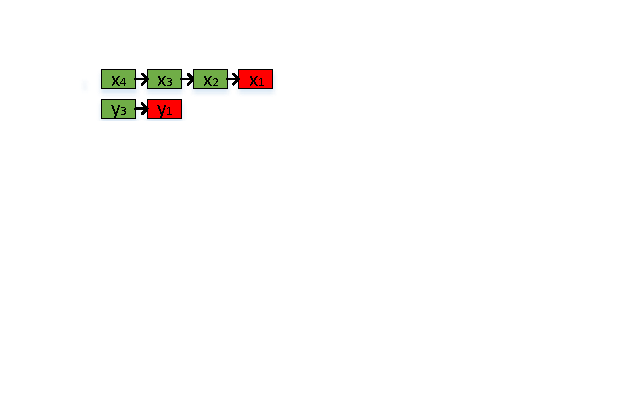
\includegraphics[scale=1.5] {figure/version1} \label{fig:versions_a}}
    \captionsetup[subfigure]{margin={0cm,0cm}
  }
  \subfloat[\small ${H_b = H_a c_2r_5[y_3]w_6[x_4]}$]
  {
    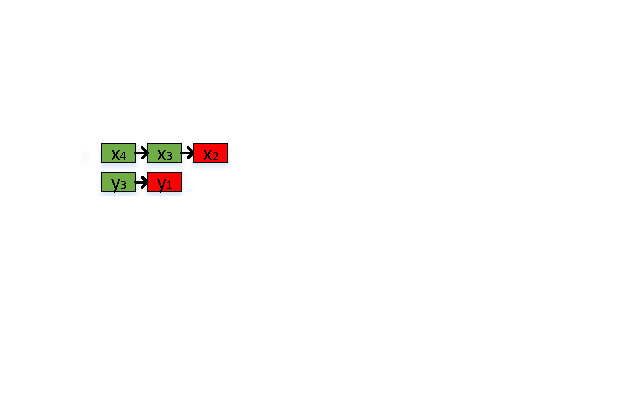
\includegraphics[scale=1.5]{figure/version2} \label{fig:versions_b}
  }
    \captionsetup[subfigure]{margin={0cm,0cm}
  }
  \subfloat[\small ${H_c = H_b a_3a_5}$]
  {
    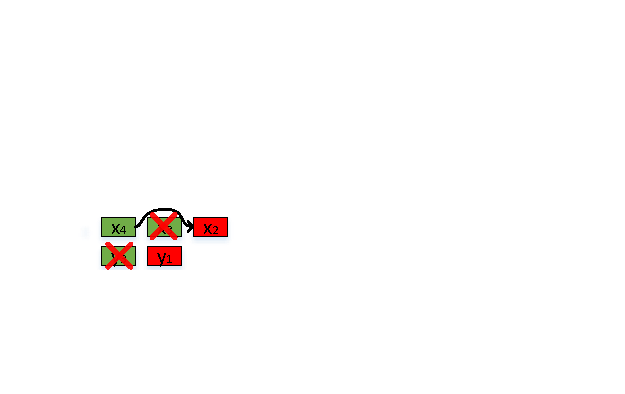
\includegraphics[scale=1.5] {figure/version3} \label{fig:versions_c}}
    \captionsetup[subfigure]{margin={0cm,0cm}}
    \subfloat[\small ${H_d = H_c c_4r_6[y_1]c_6}$]
      { 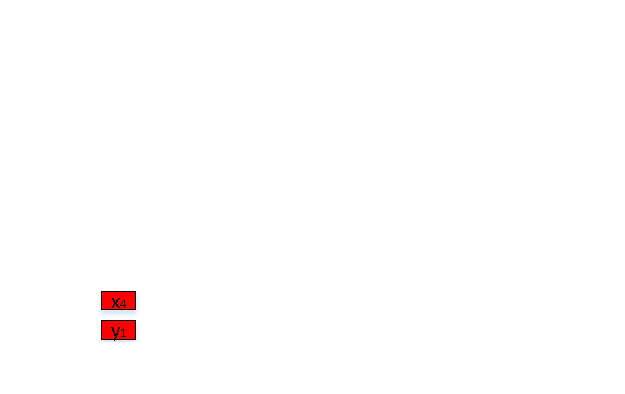
\includegraphics[scale=1.5]{figure/version4} \label{fig:versions_d}
  }
  \caption{\emph{ww}-dependencies are not required for recovery.
  ${x_i}$ represents the version of $x$ created by ${T_i}$.
 Then, $w_j[x_i]$ represents that ${T_j}$ overwrites the write of ${T_i}$ on $x$.
}
\label{fig:versions_example}
\end{figure}


\subsection {Deadlock Handling}
There are various approaches to handle deadlock.
We choose two typical ones to discuss how lock violation can adapt to deadlock handle.

Deadlock detection is most widely used by centralized DB.
Deadlock detection strategies are generally
based on tracing waits-for graph (WFG).
DLV implement non-centralized deadlock detection use \emph{path pushing} approach . %TODO
For early violation, 
only the truely locking wait transactions but also lock violation transactions would contribute edges to WFG. 
Additional edges in WFG at any time, in turn, lead  more likely deadlock and greater abort rate.
Late violation would not violate serializability and violation action need not be traced by deadlock detection.

Another approach to handle deadlocks is deadlock prevention.
We adopts the \emph{wait-die} protocol to prevent deadlocks and preserve serializability.
A transaction is assigned a unique timestamp when it starts.
(This does not require a centralized timestamp allocator.
Each node can generate a unique timestamp for its transactions by combining its local clock time and its node id.)
Then, conflicting transactions can be ordered by their timestamps.
Following the wait-die protocol, a transaction will wait if it attempts to access a data item locked by a transaction with a larger timestamp.
If the item is locked by a transaction with a smaller timestamp, it will abort.
By only allowing a transaction to violate a lock with greater transaction id, 
it can guarantee that the data dependencies are acyclic.
Similar deadlock detection approach,
early lock violation scheduler must apply the \emph{wait-die} protocol for violaiton action to ensure serializability, but it is not necessary for late violation.


\section{Experiments and Evaluations}
\label{sec:experiments}
We developed a GDDB engine to evaluate the performance of \emph{DLV}.
We compared different types of \emph{DLV} against the traditional S2PL approach. 
In the implementation of S2PL, we used the wait-die policy to resolve deadlocks, as it is known as one of the most efficient approaches in geo-distributed databases.
When the wait-die policy is employed, aborts, instead of blocking, will be the main obstacle of performance. 

\subsection{Experimental Setting}
\label{subsec:exp_setting}
Our experiments were performed on a cluster of 13 Aliyun ecs.g6.3xlarge servers.
Each server was equipped with 12 virtual CPU cores of 2.5GHz and a 48GiB RAM. The OS was Ubuntu 18.04.
Twelve of the servers were used to deploy the transaction engine.
The data were partitioned into 4 shards. 
Each shard had 3 replicas spread across 3 AZs, 
which were located at Heyuan (South China), Hangzhou (East China), and Zhangjiakou (North China).
Every AZ had a full copy of each shard of data.
The internal network bandwidth in each AZ was 1Gbps.
One of the servers was used as the client node, dedicated to issuing transaction requests. 
In the experiments, if a transaction aborted due to confliction, it would be retried in 2 seconds.
We used the TPC-C and YCSB benchmarks to perform the evaluation. 


TPC-C~\cite{TPCC:conf/tpctc/NambiarWMTLCM11} models a real-world scenario, in which a company sells products through multiple warehouses in different districts, and customers order products and pay bills.
In our version of TPC-C, we partitioned the data into 4 shards mainly by the warehouse IDs.
The item table was replicated across all the shards.
As our purpose was to evaluate the performance of distributed transactions,
we made all the transactions distributed by enforcing each transaction to order items from warehouses located at different nodes.
We excluded the think time, and only measured the performance of the NewOrder transactions.


YCSB~\cite{YCSB:conf/cloud/CooperSTRS10} was originally designed to evaluate NoSQL databases.
Its transactions are relatively simple.
Each YCSB transaction accesses nearly 10 rows of data according to a Zipfian distribution.
By adjusting the degree of skewness of the Zipfian (i.e., the parameter \emph{theta}), we can customize the degree of contention.
We partitioned the YCSB data by the primary key of the main table.
To make all transactions distributed, we forced each transaction to access at least two shards.

Table~\ref{tbl:metric} shows the metrics we used in our evaluation.

\newcommand{\tabincell}[2]{\begin{tabular}{@{}#1@{}}#2\end{tabular}}
\begin{table}[htb]
  \centering
  \begin{tabular}{|r|c|}
  \hline
Metric & \tabincell{c}{Definition}   \\
  \hline
  \hline
  TPM & \tabincell{c}{ the number of transactions committed in each minute}  \\
  \hline
  Abort Rate & \tabincell{c}{the proportion of transactions that fail to commit }  \\
  \hline
  \end{tabular}
\caption{Metrics for Evaluation }
\label{tbl:metric}
\end{table}

\subsection{Impact of Geo-replication}

In the first set of experiments, we evaluated how geo-replication affects the performance of transaction processing.
We simulated geo-replication in a single AZ. 
Namely, we put all replicas in the same AZ and artificially increased the communication latency among the replicas. 
We used the TPC-C workload, in which we set the number of warehouses to 20 and the number of concurrent clients connected to each shard to 100.
Fig.~\ref{fig:new_order_add_log_cost} shows how the throughput and the abort rate of TPC-C changed with the increased replication latency.
Geo-replication has a great impact on performance. The higher the replication latency, the lower the throughput of transaction processing.

We can also see that the DLVs performed significantly better than traditional S2PL in the experiments.
DLV1x outperformed S2PL by 2-3 times when the replication latency is high.
As all the candidate schedulers adopted the wait-die policy, transactions normally chose to abort when confronted with serious contention.
Therefore, the abort rates measure how the performance was affected by contention.
The result shows that DLV1x and DLV2 could deal with contention better than the others.
As they release locks earlier than S2PL, they are subject to less contention than S2PL. (DLV1x releases locks earlier than DLV2.) 
While DLV0 and DLV1 perform lock violation too, they suffer from an increased chance of serializability breach and cascade aborts.
Therefore, their abort rates were also high in the experiments.

\begin{figure}[htbp]
  %cloud setting
  \centering
  \captionsetup[subfigure]{margin={0cm,0cm}}
  \subfloat[NewOrder TPM]
      { 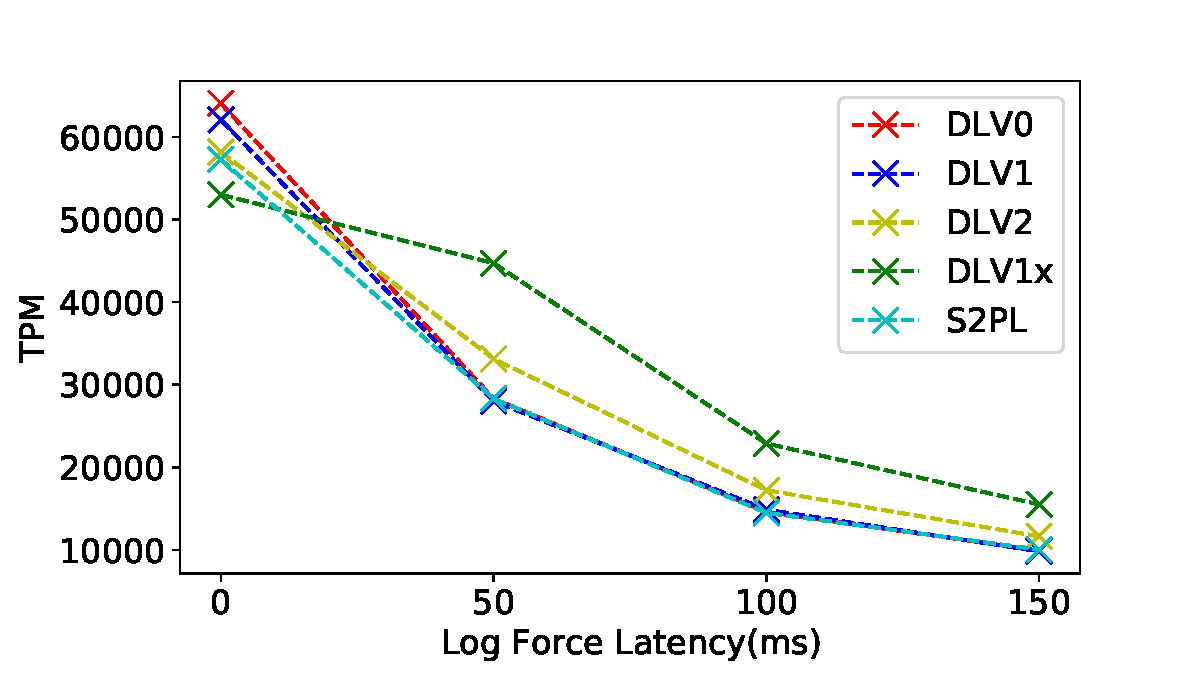
\includegraphics[scale=0.4] {figure/plot_tpcc_neworder_add_LogForceT_LogForceT_TPM_gather} \label{fig:new_order_add_log_cost:tpm}}
  
  \captionsetup[subfigure]{margin={0cm,0cm}}
  \subfloat[NewOrder abort rate]
      { 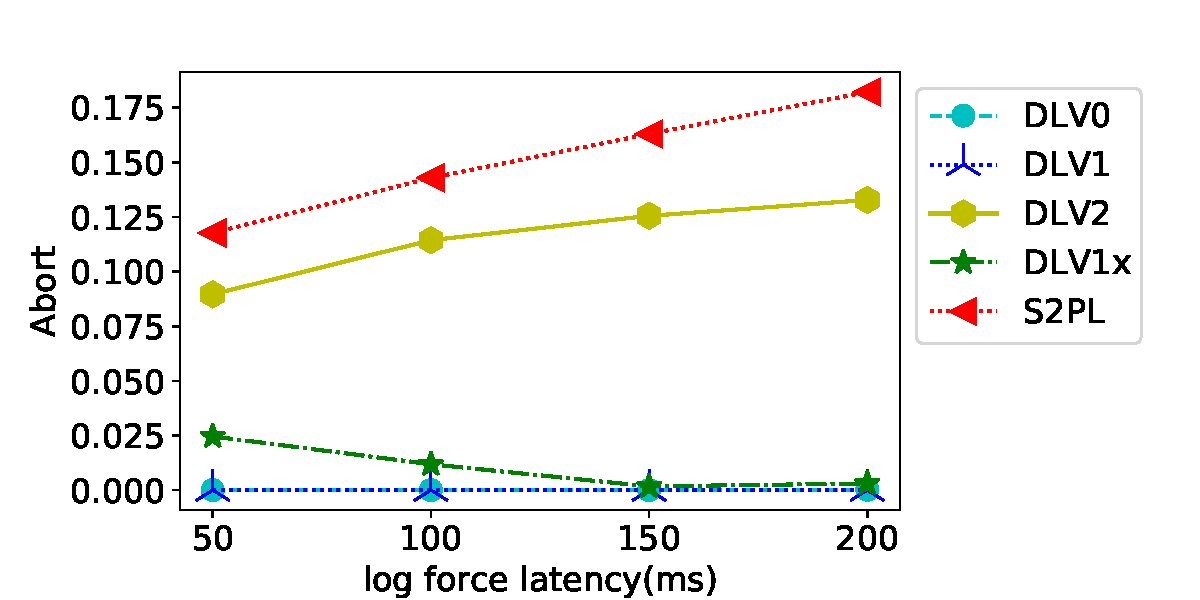
\includegraphics[scale=0.4]{figure/plot_tpcc_neworder_add_LogForceT_LogForceT_Abort_gather} \label{fig:new_order_add_log_cost:abort}}

\caption{throughput and abort rate of
different terminal different log write costs}
\label{fig:new_order_add_log_cost}
\end{figure}


\subsection{Impact of Contention}

Our second set of experiments aim to evaluate how the degree of contention affects the performance of transaction processing.
We used both the TPC-C workload and the YCSB workload.
We ran all the experiments in a real geo-replication environment described in Section~\ref{subsec:exp_setting}.
In the experiments, we adopted the gathered mode, which assumes that all replica leaders co-locate in the same AZ. 


\begin{figure}[htbp]
  \centering
  \captionsetup[subfigure]{margin={0cm,0cm}}
  \subfloat[NewOrder TPM]
      { 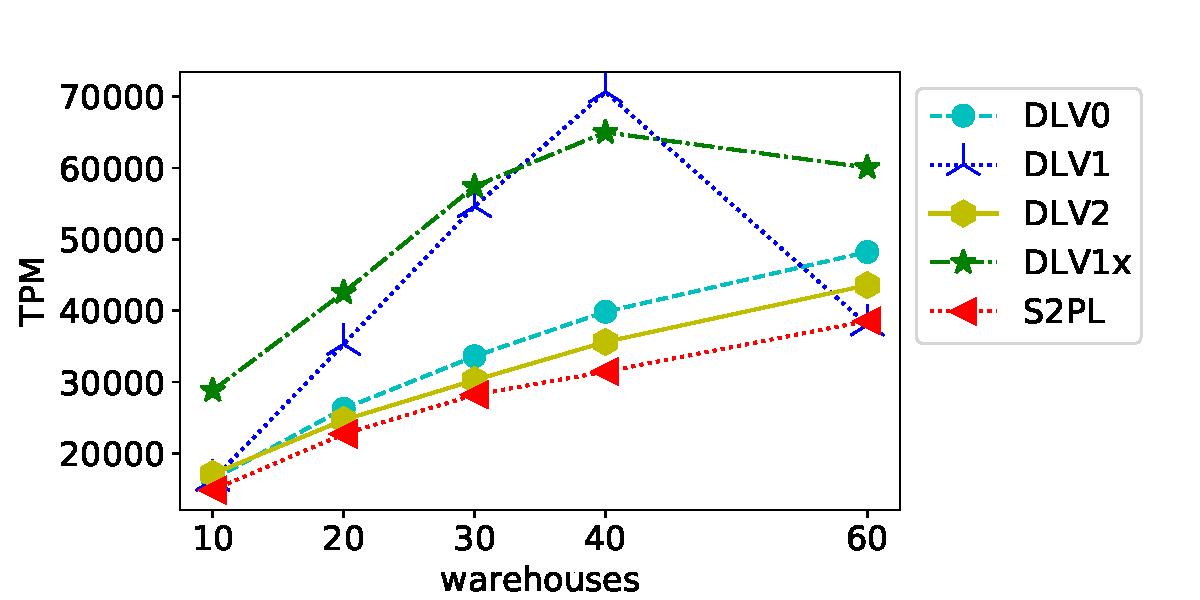
\includegraphics[scale=0.4] {figure/plot_tpcc_neworder_add_Warehouse_Warehouse_TPM_gather} \label{fig:plot_tpcc_neworder_add_Warehouse_Warehouse_gather:tpm}}
  \captionsetup[subfigure]{margin={0cm,0cm}}
  \subfloat[NewOrder abort rate]
      { 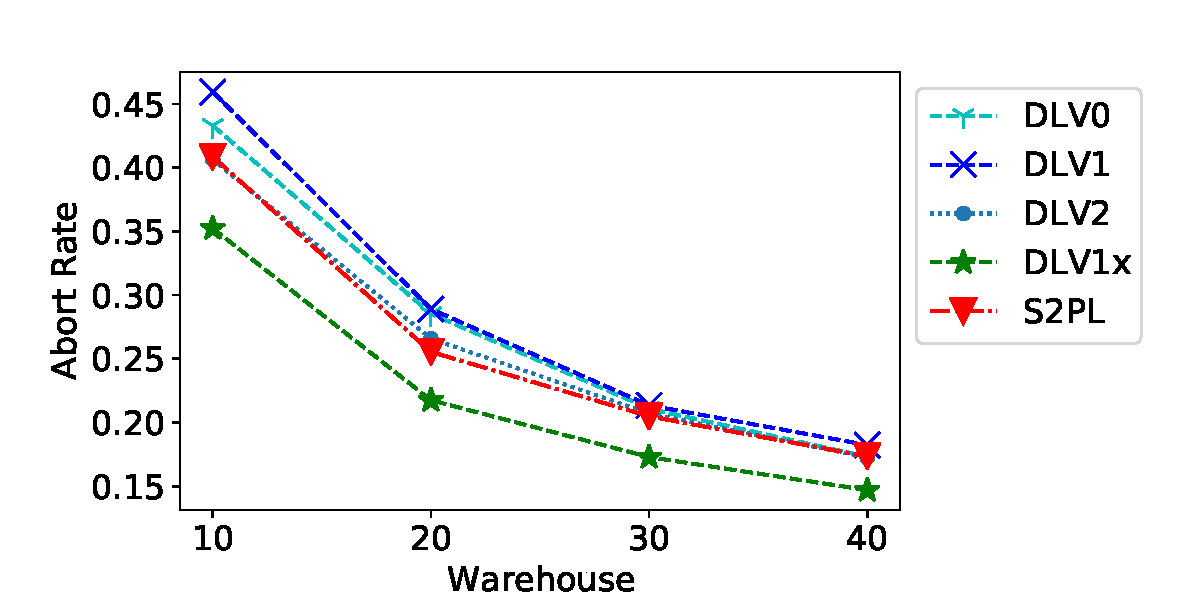
\includegraphics[scale=0.4]{figure/plot_tpcc_neworder_add_Warehouse_Warehouse_Abort_gather} \label{fig:plot_tpcc_neworder_add_Warehouse_Warehouse_gather:abort}}      
\caption{throughput and abort rate of different warehouses}
\label{fig:plot_tpcc_neworder_add_Warehouse_Warehouse_gather}
\end{figure}

\begin{figure}[htbp]
  \centering
  \captionsetup[subfigure]{margin={0cm,0cm}}
  \subfloat[NewOrder TPM]
      { 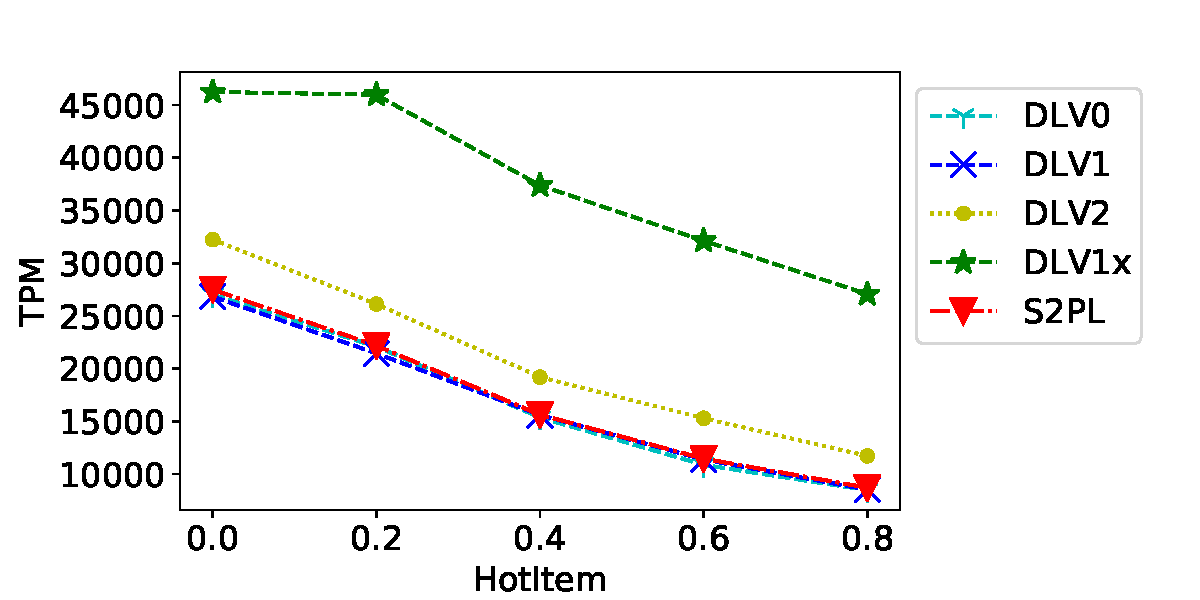
\includegraphics[scale=0.4] {figure/plot_tpcc_neworder_add_HotItem_HotItem_TPM_gather} \label{fig:plot_tpcc_neworder_add_HotItem_HotItem_gather:tpm}}
  \captionsetup[subfigure]{margin={0cm,0cm}}
  \subfloat[NewOrder abort rate]
      { 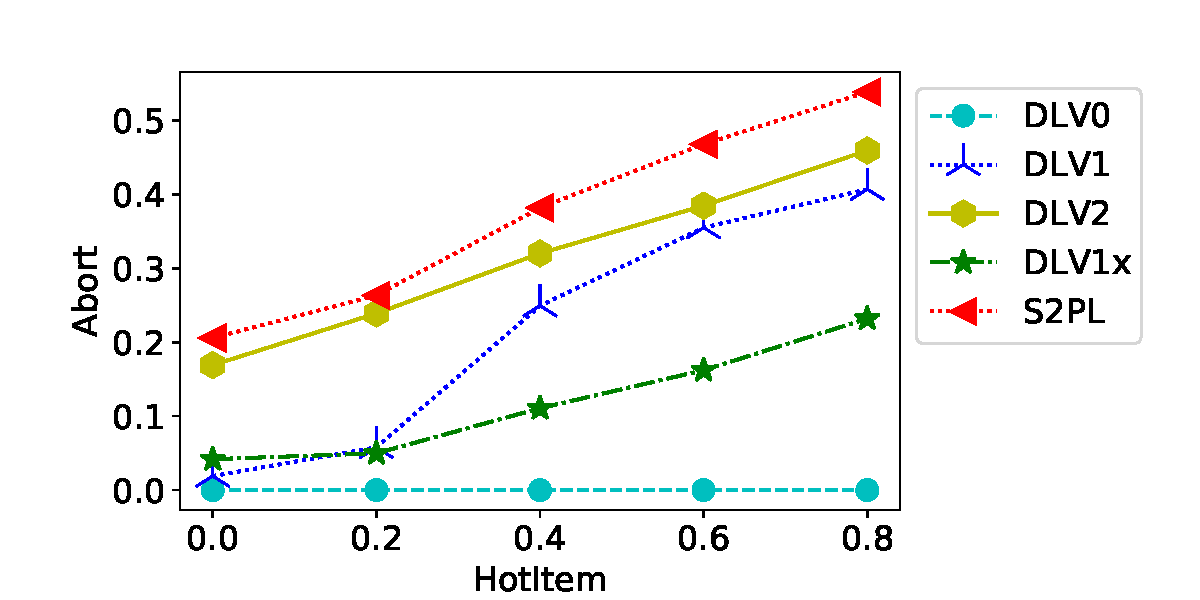
\includegraphics[scale=0.4]{figure/plot_tpcc_neworder_add_HotItem_HotItem_Abort_gather} \label{fig:plot_tpcc_neworder_add_HotItem_HotItem_gather:abort}}
\caption{throughput and abort rate of various percent of the transaction request accessing hot rows}
\label{fig:plot_tpcc_neworder_add_HotItem_HotItem_gather}
\end{figure}

In Fig.~\ref{fig:plot_tpcc_neworder_add_Warehouse_Warehouse_gather}, we fixed the number of clients of every shard to 100 and varied the number of warehouses between 10 to 60.
The smaller the number of warehouses, the higher the degree of contention. 
As we can see, when the number of warehouses was 10, DLV outperformed S2PL by up to 2 times.

Fig.~\ref{fig:plot_tpcc_neworder_add_HotItem_HotItem_gather} shows how the throughput of transaction processing varied according to the percent of the transaction request accessing hot rows.
The performance of DLV is 3 times higher than that of S2PL when the possibility of the transaction accessing hotspot reaches 0.8.

From Fig.~\ref{fig:plot_tpcc_neworder_add_Warehouse_Warehouse_gather} and 
Fig.~\ref{fig:plot_tpcc_neworder_add_HotItem_HotItem_gather}, 
we can see that contention had a big impact on performance. When the degree of contention decreased, the throughput rose quickly.
The DLVs performed better than S2PL in general, as lock violation had shortened their lock holding time, especially when the degree of contention is high. 
DLV0 and DLV1 do not improve throughput a great because it has a more abort rate than S2PL.
Among the DLVs, DLV1x performed the best, as it suffered less from blocking conflicts locks and cascade aborts.

\begin{figure}[htbp]
  \centering
  \captionsetup[subfigure]{margin={0cm,0cm}}
  \subfloat[YCSB workload TPM]
      { 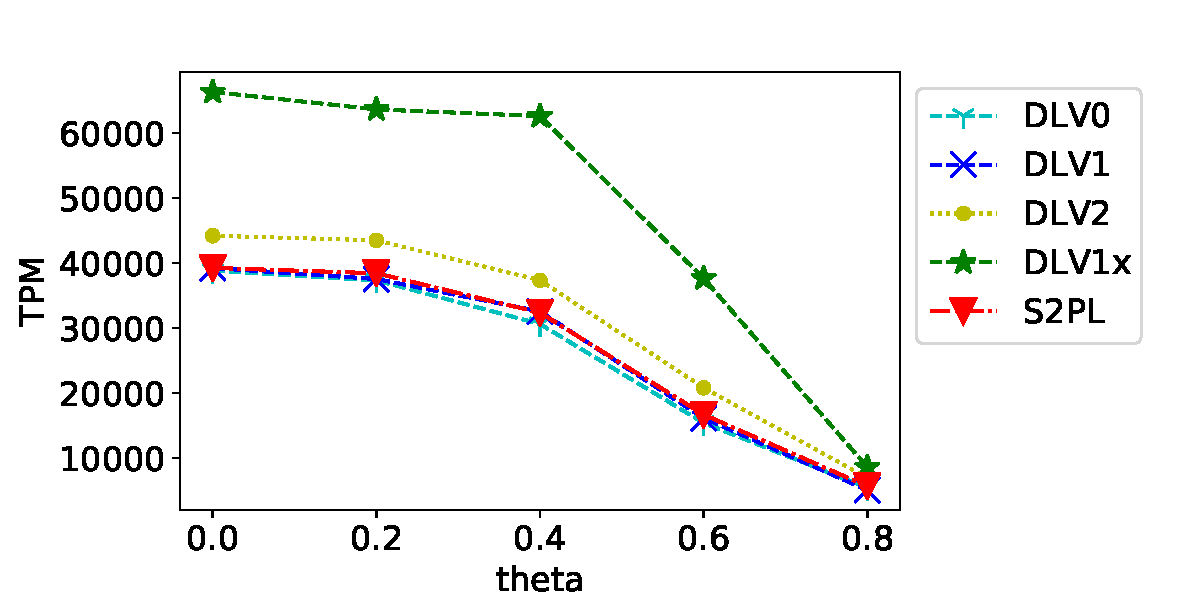
\includegraphics[scale=0.4] {figure/plot_ycsb_add_Theta_Theta_TPM_gather} \label{fig:plot_ycsb_add_Theta_Theta_TPM_gather:tpm}}
  
      \captionsetup[subfigure]{margin={0cm,0cm}}
  \subfloat[YCSB workload abort rate]
      { 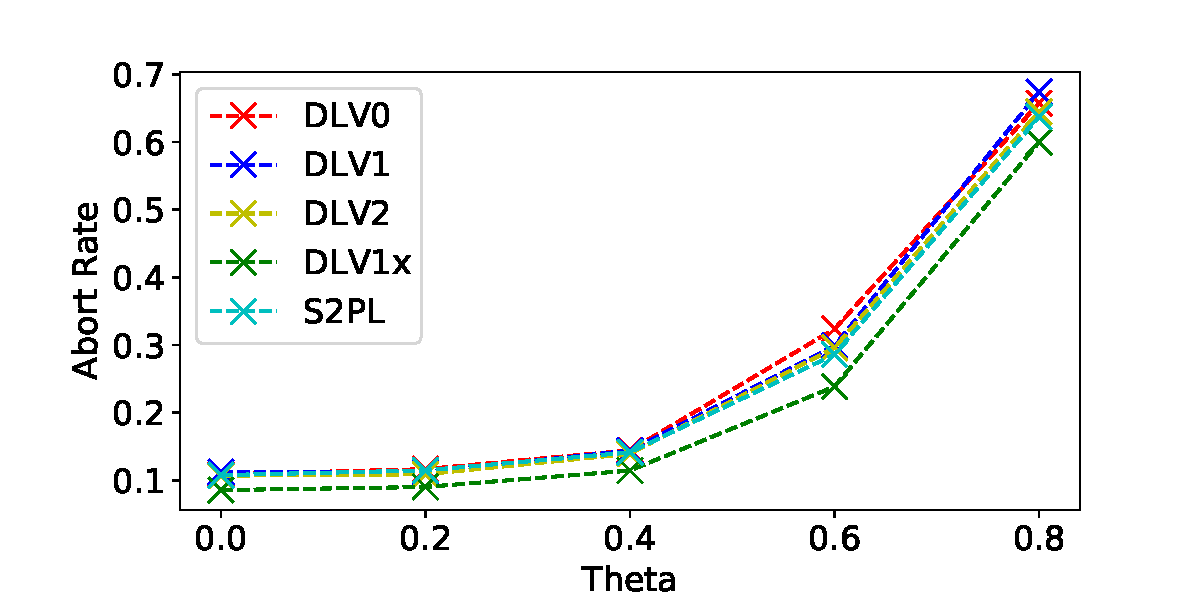
\includegraphics[scale=0.4]{figure/plot_ycsb_add_Theta_Theta_Abort_gather.pdf} \label{fig:plot_ycsb_add_Theta_Theta_TPM_gather:abort}}


\caption{YCSB performance, throughput and abort rate when adding theta, in gathered mode}
\label{fig:plot_ycsb_add_Theta_Theta_TPM_gather}
\end{figure}

In the experiments on YCSB, we fixed the number of clients of every shard to 100.
Then we varied the parameter \emph{theta} (the skewness of the Zipfian distribution) to control the degree of contention and evaluate the performance.
The larger the \emph{theta}, the more skewed the distribution and the higher the degree of contention. 
Fig. ~\ref{fig:plot_ycsb_add_Theta_Theta_TPM_gather} shows how the throughput was affected by the changing skewness.
The results also show that contention had a huge impact on performance.
Similar to the results on TPC-C, DLVs outperformed S2PL, and DLV1x performed the best.

\subsection{On Scalability}

To evaluate the scalability of distributed transactions, we conducted experiments in both the gathered mode and the scattered mode.
In the gathered mode, all the replica leaders are in the same AZ. 
The gathered mode is the most common mode, in which servers in the leaders' AZ served the requests mainly, and servers in other AZs are for the replication purpose only. 
In the scattered mode, the replica leaders may spread across different AZs. 
Large-scale Web applications usually adopt this mode, which intentionally makes their service available everywhere.

We conducted experiments on TPC-C and YCSB workloads. 
Fig. ~\ref{fig:new_order_add_terminal_gathered} shows the performance of distributed transactions on TPC-C workload in the gathered mode.
We fixed the number of warehouses to 40. 
Then we gradually increased the number of clients until the system was saturated. 
We can see that DLVs outperformed S2PL in general. 
The maximum throughput S2PL could achieve around 31,000 TPM (Transactions per Minute), 
while the throughput of DLV1x could achieve 59,000 TPM.


Fig. ~\ref{fig:new_order_add_terminal_scattered}  shows the TPC-C evaluation results in the scattered mode. 
As the intra-transaction communication in the scattered mode needs to cross AZs, its performance was slightly worse than that of the gathered mode.
Nevertheless, the results exhibit the same trend. DLVs outperformed S2PL significantly.

We also evaluate the throughput on YCSB when increasing the terminal number of each shard.
Fig. ~\ref{fig:ycsb_add_terminal_gathered} shows the results.
DLV1x scales better when adding concurrent terminals.
When the test reaches the maximum number of concurrent terminals, the throughput of DLV1x is twice as that of S2PL.

\begin{figure}[htbp]
  \centering
  \captionsetup[subfigure]{margin={0cm,0cm}}
  \subfloat[NewOrder TPM]
      { 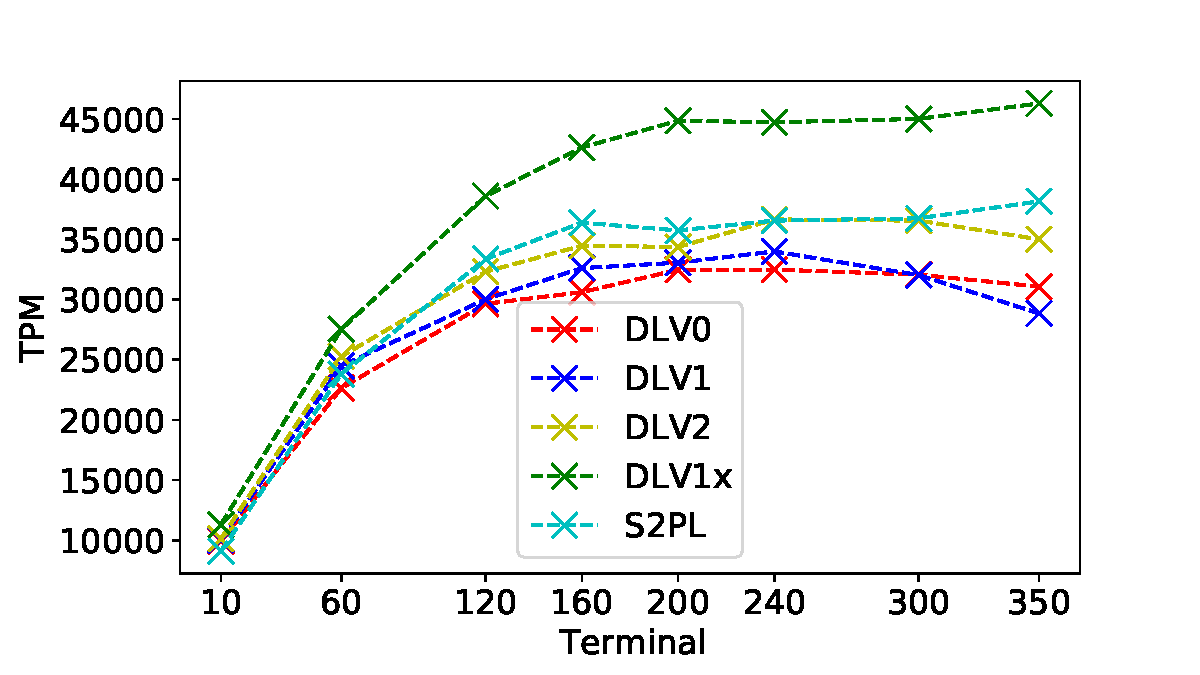
\includegraphics[scale=0.4] {figure/plot_tpcc_neworder_add_Terminal_Terminal_TPM_gather} \label{fig:new_order_add_terminal_gathered:tpm}}
  
      \captionsetup[subfigure]{margin={0cm,0cm}}
  \subfloat[NewOrder abort rate]
      { 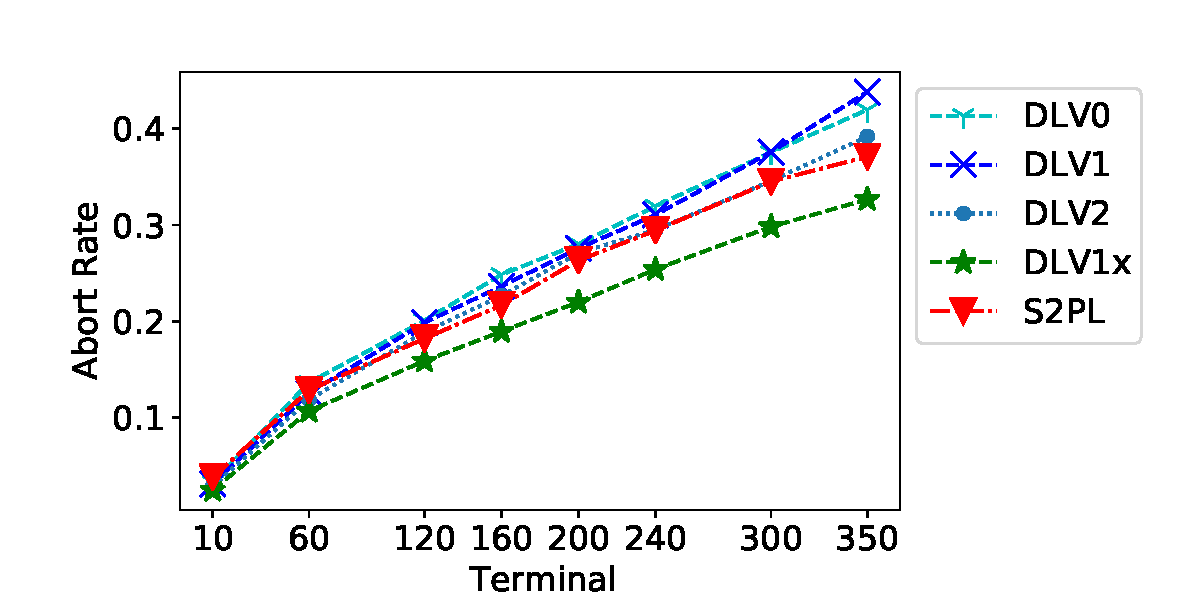
\includegraphics[scale=0.4]{figure/plot_tpcc_neworder_add_Terminal_Terminal_Abort_gather} \label{fig:new_order_add_terminal_gathered:abort}}

\caption{throughput and abort rate when adding terminals, in gathered mode}
\label{fig:new_order_add_terminal_gathered}
\end{figure}

\begin{figure}[htbp]
  \centering
  \captionsetup[subfigure]{margin={0cm,0cm}}
  \subfloat[NewOrder TPM]
      { 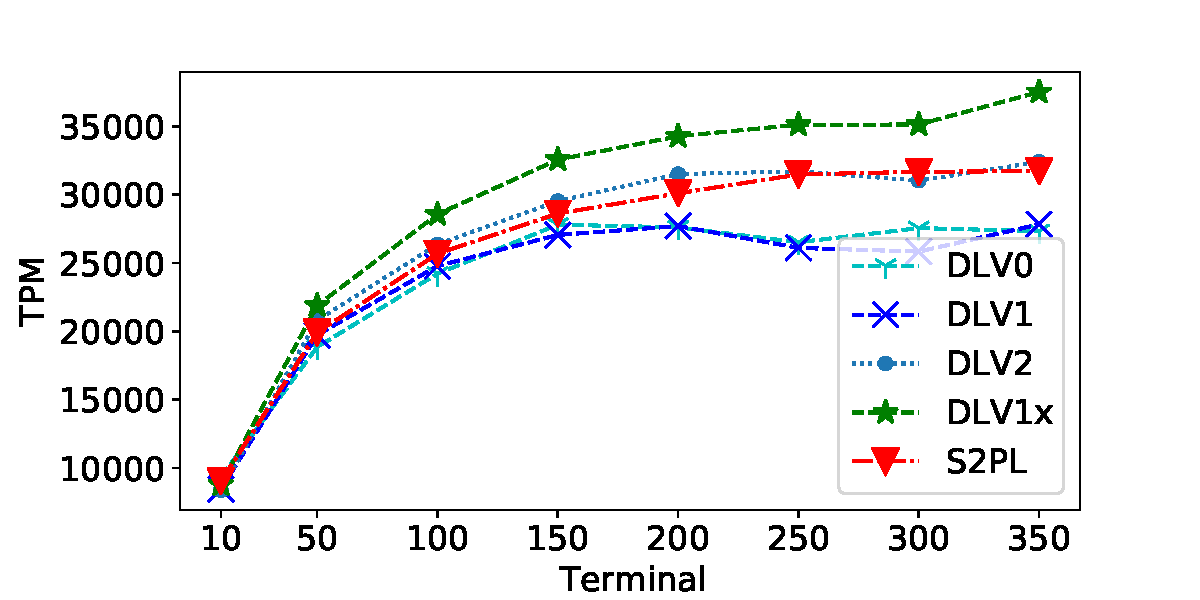
\includegraphics[scale=0.4] {figure/plot_tpcc_neworder_add_Terminal_Terminal_TPM_scatter} \label{fig:new_order_add_terminal_scattered:tpm}}
  
      \captionsetup[subfigure]{margin={0cm,0cm}}
  \subfloat[NewOrder abort rate]
      { 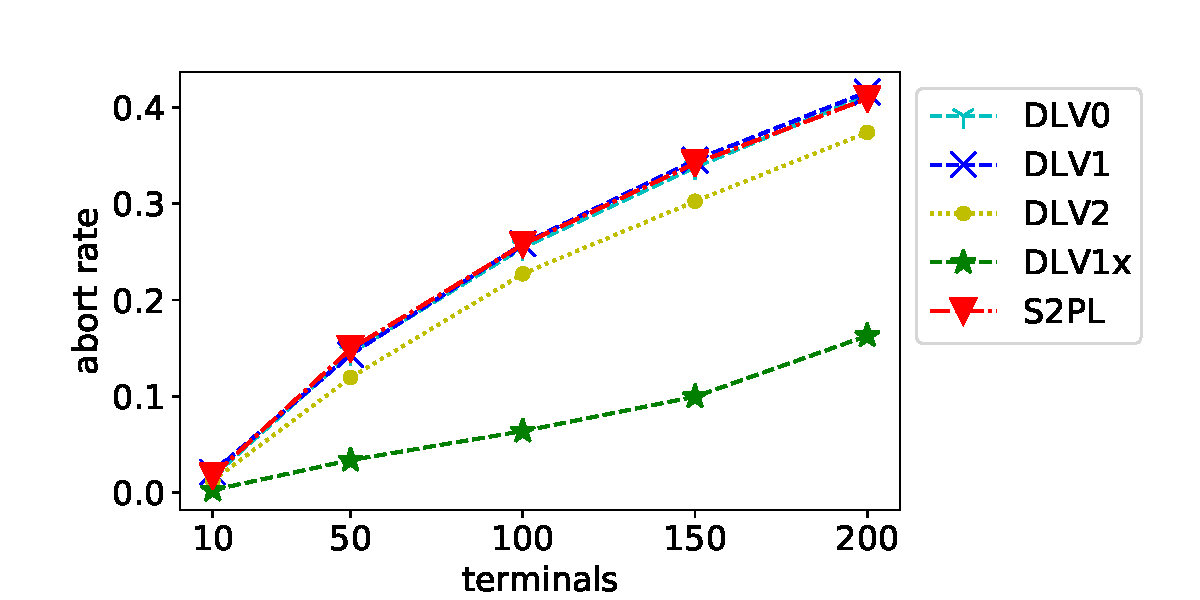
\includegraphics[scale=0.4]{figure/plot_tpcc_neworder_add_Terminal_Terminal_Abort_scatter} \label{fig:new_order_add_terminal_scattered:abort}}

\caption{throughput and abort rate when adding terminals, in scattered mode}
\label{fig:new_order_add_terminal_scattered}
\end{figure}

\begin{figure}[htbp]
  \centering
  \captionsetup[subfigure]{margin={0cm,0cm}}
  \subfloat[YCSB TPM]
      { 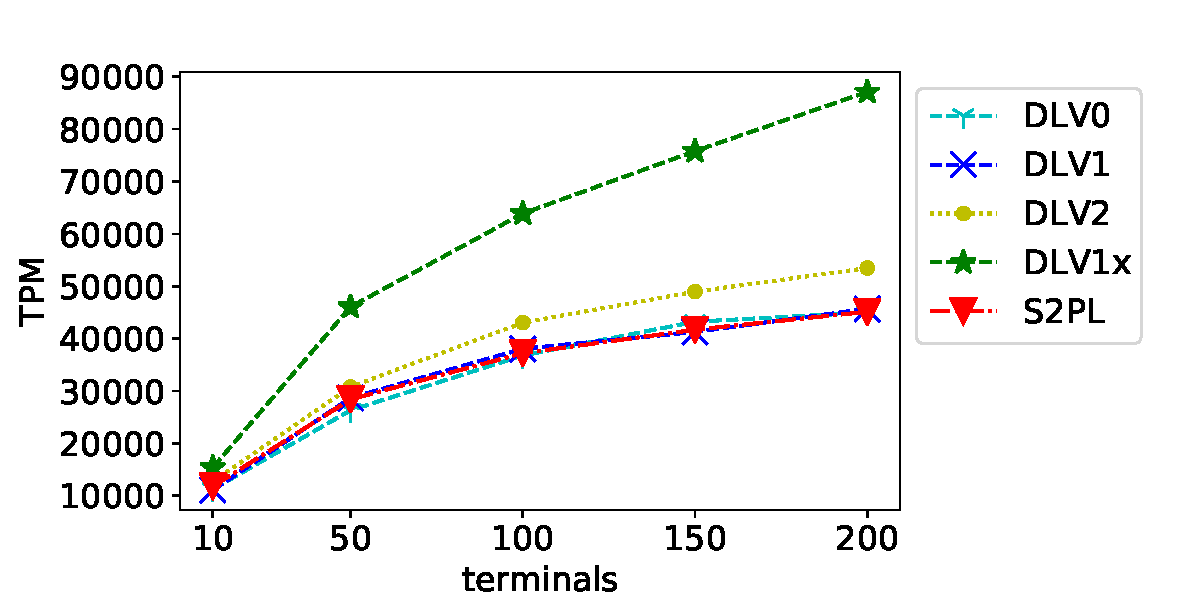
\includegraphics[scale=0.4] {figure/plot_ycsb_add_Terminal_Terminal_TPM_gather} \label{fig:ycsb_add_terminal_gathered:tpm}}
  
      \captionsetup[subfigure]{margin={0cm,0cm}}
  \subfloat[YCSB abort rate]
      { 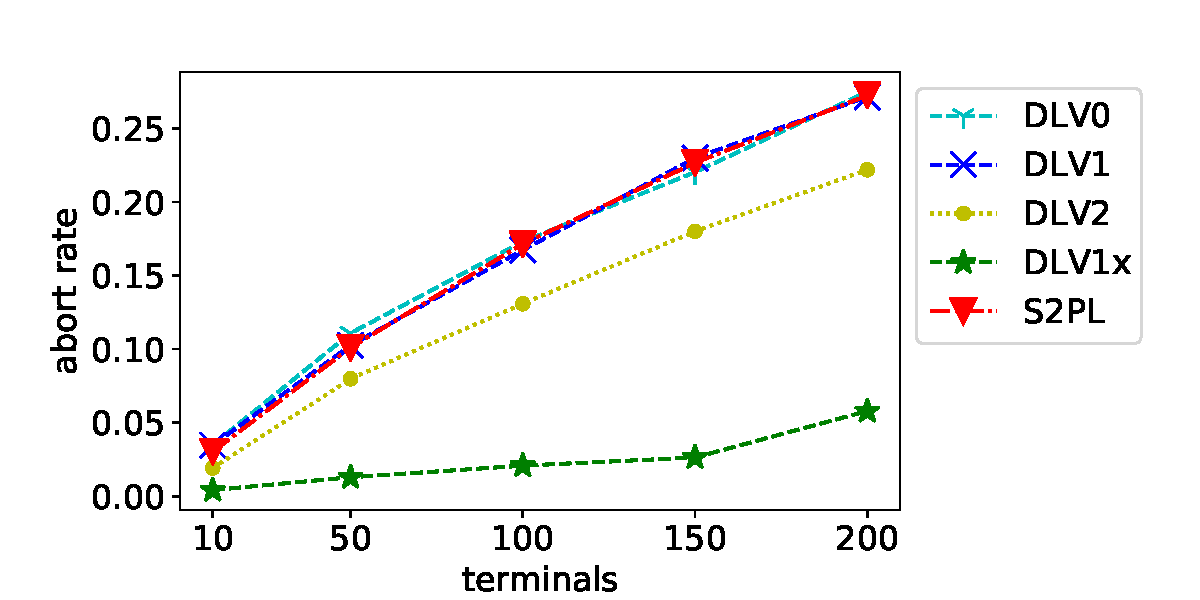
\includegraphics[scale=0.4]{figure/plot_ycsb_add_Terminal_Terminal_Abort_gather} \label{fig:ycsb_add_terminal_gathered:abort}}


\caption{throughput and abort rate when adding terminal number of each shard, in gathered mode}
\label{fig:ycsb_add_terminal_gathered}
\end{figure}


\begin{figure}[htbp]
  \centering
  \captionsetup[subfigure]{margin={0cm,0cm}}
  { 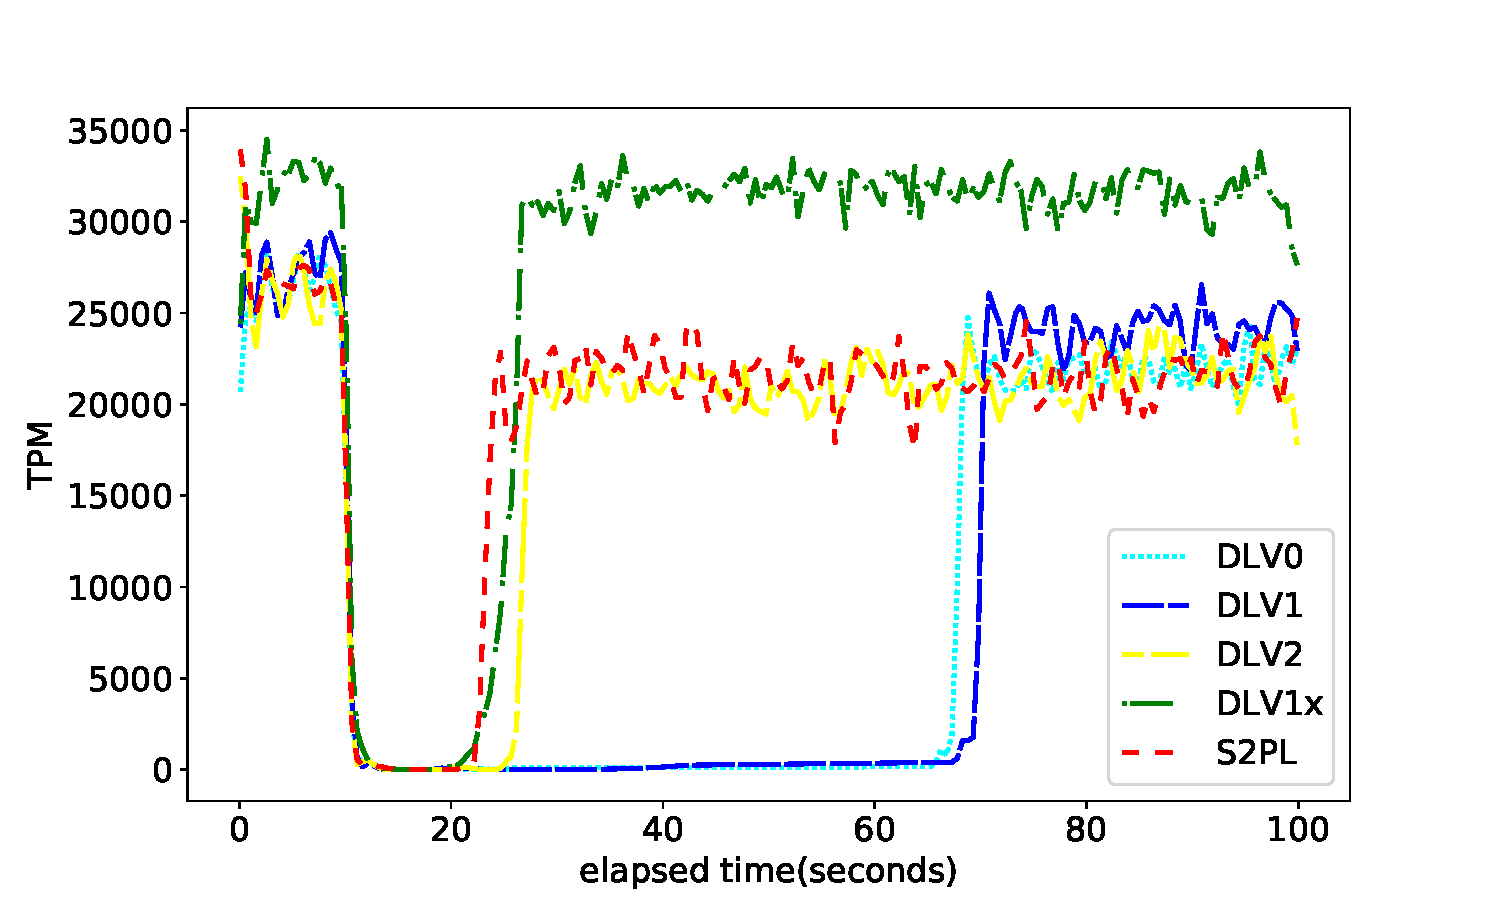
\includegraphics[scale=0.36] {figure/plot_availability} 
  \caption{non availability time after one AZ is down}
  \label{fig:plot_availability:tpm}}
\end{figure}

\subsection{Non-availability Time After Failure}

Due to speculation and cascade abort, the database would take more time to abort running transactions when a failure occurs.
In our final evaluation of our experiments, we evaluate the non-availability time of different algorithms after an AZ failure.
Fig~\ref{fig:plot_availability:tpm} shows how throughput changes over time elapsed during one AZ failure.
This result shows DLV0, DLV1 endures longer non-available time after an AZ failure.
DLV2 and DLV1x have less non-available time for less false positive speculation.


\subsection{Experimental Conclusion}

In conclusion, our experimental evaluation showed that the geo-replication can have a big negative impact on the performance of distributed transactions.
Besides the overheads of data synchronization incurred by replication, the prolonged lock holding time is also a main contributor to the degraded performance.
We demonstrated that lock violation can be an effective measure to shorten the lock holding time and thus boost the performance of GDDB.
To harness the benefit of lock violation, it is important to find the right time to release the locks.
Our evaluation also showed that late lock violation is superior to early lock violation in most cases, as it is much less prone to high abort rates.


\section{Conclusion}
\label{sec:conclusion}

This paper discussed the application of lock violation in geo-replicated distributed databases.
Lock violation is not only concerned with the concurrency control mechanism, but it is also related to the modules of recovery and persistence.
Therefore, its adoption requires a holistic redesign of the transaction processor. 
In this paper, we proposed such a holistic design and conducted experiments to evaluate its effectiveness.
The results showed that lock violation can boost the performance of a geo-replicated distributed database, especially when the degree of contention is high.
Moreover, we found that not all lock violation approaches can be beneficial. We identified the right time to perform violation, so as to maximize its effects. 

Distributed transaction remains a challenge to our research community. Recent progress of the HA technologies has made distributed transactions less vulnerable to failures.
However, the performance of distributed transactions in general still falls short of the requirements of many mission-critical applications.
While lock violation is an effective technique to optimize distributed transactions, it is far from an ultimate solution.
As we can see in our experimental evaluation, even with this optimization, the general performance of distributed transactions is sometimes unsatisfactory.
Considering the ever-increasing scale of modern Web applications, We believe that further research on distributed transaction is not only necessary but important.

\bibliographystyle{reference/IEEEtran}
\bibliography{reference/IEEEexample}

 
\end{document}

